% -*- TeX:UTF-8 -*-
%%
%% KAIST 학위논문양식 LaTeX용 (ver 0.4) 예시
%%
%% @version 0.4
%% @author  채승병 Chae,Seungbyung (mailto:chess@kaist.ac.kr)
%% @date    2004. 11. 12.
%%
%% @requirement
%% teTeX, fpTeX, teTeX 등의 LaTeX2e 배포판
%% + 은광희 님의 HLaTeX 0.991 이상 버젼 또는 홍석호 님의 HPACK 1.0
%% : 설치에 대한 자세한 정보는 http://www.ktug.or.kr을 참조바랍니다.
%%
%% @note
%% 기존에 널리 쓰여오던 차재춘 님의 학위논문양식 클래스 파일의 형식을
%% 따르지 않고 전면적으로 다시 작성하였습니다. 논문 정보 입력부분에서
%% 과거 양식과 다른 부분이 많으니 아래 예시에 맞춰 바꿔주십시오.
%%
%%
%% @acknowledgement
%% 본 예시 논문은 물리학과 박사과정 김용현 님의 호의로 제공되었습니다.
%%
%% -------------------------------------------------------------------
%% @information
%% 이 예제 파일은 hangul-ucs를 사용합니다. UTF-8 입력 인코딩으로
%% 작성되었습니다. hlatex의 hfont는 이용하지 않습니다. --2006/02/11

% @class kaist.cls
% @options [default: doctor, korean, final]
% - doctor: 박사과정 | master : 석사과정
% - korean: 한글논문 | english: 영문논문
% - final : 최종판   | draft  : 시험판
% - pdfdoc : 선택하지 않으면 북마크와 colorlink를 만들지 않습니다.

%% 마지막엔 final로 해서 표지까지 다 나오도록
\documentclass[master,english,final]{kaist-ucs}
% \documentclass[master,english,draft]{kaist-ucs}


% If you want make pdf document (include bookmark, colorlink)
%\documentclass[doctor,english,final,pdfdoc]{kaist-ucs}

% kaist.cls 에서는 기본으로 dhucs, ifpdf, graphicx 패키지가 로드됩니다.
% 추가로 필요한 패키지가 있다면 주석을 풀고 적어넣으십시오,
%\usepackage{...}
\usepackage{amsfonts}
\usepackage{bm}
\usepackage{multirow}
\usepackage{amsmath}
\usepackage{algorithm}
\usepackage{algpseudocode}
% \usepackage{subfigure}
\usepackage{subcaption}

\makeatletter
\renewcommand{\Function}[2]{%
  \csname ALG@cmd@\ALG@L @Function\endcsname{#1}{#2}%
  \def\jayden@currentfunction{#1}%
}
\newcommand{\funclabel}[1]{%
  \@bsphack
  \protected@write\@auxout{}{%
    \string\newlabel{#1}{{\jayden@currentfunction}{\thepage}}%
  }%
  \@esphack
}
\makeatother

% @command title 논문 제목(title of thesis)
% @options [default: (none)]
% - korean: 한글제목(korean title) | english: 영문제목(english title)
\title[korean] {상품 평가 품질 조작에 견고한 추천 시스템}
\title[english]{A Robust Recommendation System \linebreak Against Review Quality Manipulation}

% @note 표지에 출력되는 제목을 강제로 줄바꿈하려면 \linebreak 을 삽입.
%       \\ 나 \newline 등을 사용하면 안됩니다. (아래는 예시)
%
%\title[korean]{탄소 나노튜브의 물리적 특성에 대한\linebreak 이론 연구}
%\title[english]{Theoretical study on physical properties of\linebreak
%                carbon nanotubes}
%
% If you want to begin a new line in cover, use \linebreak .
% See examples above.
%


% @command author 저자 이름
% @param   family_name, given_name 성, 이름을 구분해서 입력
% @options [default: (none)]
% - korean: 한글이름 | chinese: 한문이름 | english: 영문이름
% 한문 이름이 없다면 빈 칸으로 두셔도 됩니다.
%
%
% If you are a foreigner , write your name in korean or your korean name.
% If you can't write native character, you can make the chinese blank empty
% Write as follow
% \author[korean]{family name in korean}{given name in korean}
% \author[chinese]{family name in your native language}{given name in your native language}
% \author[english]{family name in english}{given name in english}
%
\author[korean] {심}{동 진}
\author[korean2] {심}{동진}    %이름을 붙여 써 주시기 바랍니다.
\author[chinese]{沈}{東 鎭}
\author[english]{Sim}{Dongjin}

% @command advisor 지도교수 이름 (복수가능)
% @usage   \advisor[options]{...한글이름...}{...영문이름...}{signed|nosign}
% @options [default: major]
% - major: 주 지도교수  | coopr: 공동 지도교수
\advisor[major]{이 윤 준}{Yoon-Joon Lee}{signed}
\advisor[major2]{이윤준}{Yoon-Joon Lee}{signed}    %한글 성과 한글 이름을 모두 붙여 써 주시기 바랍니다.
\advisorinfo{Professor of School of Computing} %제출승인서에 들어가는 교수님 정보, advisor's information
%\advisor[coopr]{홍 길 동}{Gil-Dong Hong}{nosign}
%\advisor[coopr2]{홍길동}{Gil-Dong Hong}{nosign}    %한글 성과 한글 이름을 모두 붙여 써 주시기 바랍니다.
%
% 지도교수 한글이름은 입력하지 않아도 됩니다.
% You may not input advisor's korean name
% like this \advisor[major]{}{Chang, Kee Joo}{signed}
%


% @command department {학과이름}{학위종류} - 아래 표에 따라 코드를 입력
% @command department {department code}{degree field}
%
% department code table
%
% PH        // 물리학과 Department of Physics
% MAS   // 수리과학과 Department of Mathematical Sciences
% CH    // 화학과 Department of Chemistry
% NST   // 나노과학기술대학원 Graduate School of Nanoscience & Technology
% NT        // 나노과학기술 학제전공 Nano Science and Technology Program
% BS    // 생명과학과 Department of Biological Sciences
% BIS   // 바이오및뇌공학과 Department of Bio and Brain Engineering
% MSE   // 의과학대학원 Graduate School of Medical Science and Engineering
% BM    // 의과학 학제전공 Biomedical Science and Engineering Program
% CE    // 건설및환경공학과 Department of Civil and Environmental Engineering
% ME    // 기계공학전공 Division of Mechanical Engineering
% AE    // 항공우주공학전공 Division of Aerospace Engineering
% OSE   // 해양시스템공학전공 Department of Ocean Systems Engineering
% CBE   // 생명화학공학과 Department of Chemical and Biomolecular Engineering
% MS    // 신소재공학과 Department of Materials Science and Engineering
% NQE   // 원자력 및 양자공학과 Department of Nuclear and Quantum Engineering
% EEW   // EEWS 대학원 Graduate School of EEWS
% PSE   // 고분자 학제전공 Polymer Science and Engineering Program
% SPE   // 우주탐사공학 학제전공 Space Exploration Engineering Program
% ENY   // 환경・에너지공학 학제전공 Environmental and Energy Technology Program
% MSB   // 경영과학과 Department of Management Science
% IT        // 경영과학과(IT경영학) Department of Management Science (IT Business)
% BAP   // 경영전문대학원프로그램 Master of Business Administration Program
% ITP   // 글로벌IT기술대학원프로그램 Global Information & Telecommunication Technology Program
% ITM   // 기술경영전문대학원 Graduate School of Innovation & Technology Management
% GCT   // 문화기술대학원 Graduate School of Culture Technology
% CT    // 문화기술(CT) 학제전공 Culture Technology Program
% EE    // 전기및전자공학부 Department of Electrical Engineering
% CS    // 전산학과 Department of Computer Science
% ICE   // 정보통신공학과 Department of Information and Communications Engineering
% IE        // 산업 및 시스템 공학과 Department of Industrial & Systems Engineering
% KSE   // 지식서비스공학과 Department of Knowledge Service Engineering
% ID        // 산업디자인학과 Department of Industrial Design
% RE    // 로봇공학 학제전공 Robotics Program
% STE   // 반도체 학제전공 Semiconductor Technology Educational Program
% SEP   // 소프트웨어공학프로그램 Software Engineering Program
% TE    // 정보통신공학 학제전공 Telecommunication Engineering Program
% MT    // 경영공학과 Department of Management Engineering
% TM    // 테크노경영전공 Techno-MBA Program
% FIN   // 금융전문대학원 Graduate School of Finance and Accounting
% DMP   // 디지털미디어프로그램 // Digital Media Program
% IMBA // IMBA // IMBA
% EM // 이그제큐티브MBA // Executive MBA
% SM // 사회적기업가MBA // Social Enterpreneurship MBA
% PM // 프로페셔널MBA // Professional MBA
% FEM // 금융이그제큐티브MBA // Financial Executive MBA
% GM // 녹색MBA // Green MBA
% GBP // 녹색경영정책프로그램 // Green Business and Policy Program
% IMM // 정보미디어MBA // Information and Media MBA
%
% science: 이학 | engineering: 공학 | business : 경영학
% 박사논문의 경우는 학위종류를 입력하지 않아도 됩니다.
% If you write Ph.D. dissertation, you cannot input degree field.
% The third parameter : a | b | c
% a: 소속된 학과만 쓰는 옵션 (학과에만 소속되어 있는 경우에는 무조건 a를 선택해야 함)
% b: 학과 아래의, 프로그램이나 학제전공에 소속되어 있을 경우에 학과와 프로그램을 함께 쓰는 옵션
% c: 학과 아래의, 프로그램이나 학제전공에 소속되어 있을 경우에 학과를 쓰지 않고 프로그램이나 학제전공의 이름만 쓰는 옵션
%
% a: it represents only the name of department. (if you aren't in the program under the department, must choose a)
% b: it represents the names of department and the program that is under the department (consider this when you are in the program not only department)
% c: it represents only the name of program that is under the department (consider this when you are in the program not only department)
\department{CS}{engineering}{a}

% @command studentid 학번(ID)
\studentid{20153338}

% @command referee 심사위원 (석사과정 3인, 박사과정 5인)
\referee[1]{이 윤 준}
\referee[2]{김 명 호}
\referee[3]{유 신}
%\referee[4]{가 동 호}
%\referee[5]{박 태 현}
% \referee[5] {Barack Obama}
% Of course english name is available

% @command approvaldate 지도교수논문승인일
% @param   year,month,day 연,월,일 순으로 입력
\approvaldate{December}{19}{2016}

% @command refereedate 심사위원논문심사일
% @param   year,month,day 연,월,일 순으로 입력
\refereedate{2016}{12}{19}

% @command gradyear 졸업년도
\gradyear{2017}

% 본문 시작
\begin{document}

    % 앞표지, 속표지, 학위논문 제출승인서, 학위논문 심사완료 검인서는
    % 클래스 옵션을 final로 지정해주면 자동으로 생성되며,
    % 반대로 옵션을 draft로 지정해주면 생성되지 않습니다.

    % 논문 서지, 초록, 핵심 낱말, 영문 초록, 영어 핵심 낱말 (Information of thesis, abstract in korean, keywords in korean, abstract in english, keywords in english)
   \thesisinfo
   %% Letters of abstract in korean must be less than 500 and words of abstract in english must be less than 300.
   %% Number of keywords must be less than 6.
   %% Don't write english letters in the abstract in korean.
    \begin{summary}
    추천 시스템은 사용자들의 구매 결정에 주요한 영향을 주기 때문에 악의적인 조작의 표적이 되어왔다.
    대표적인 추천 방법은 상품에 대한 평가들이 정직하다는 가정하에 사용자의 평점을 분석하는 협업 필터링 방법이다.
    하지만 협업 필터링 방법은 거짓된 평점을 주입하는 실링 공격에 의해 조작될 위험이 있다.
    이로 인해 실링 공격의 영향력을 낮추는 여러 방법이 제안되었다.
    최근에는, 많은 추천 시스템에서 사용자가 리뷰의 품질을 평가하는 점을 이용한 방법이 제안되었다..
    거짓된 리뷰는 사용자들에 의해 낮은 품질로 분류될 것이라는 가정하에 연구자들은 리뷰의 품질을 고려한 추천을 통해 실링 공격을 극복하고자 하였다.
    하지만 이러한 추천 방법은 거짓된 리뷰 품질 평가 데이터가 주입된다면 오히려 조작의 정도가 심해질 위험이 있다.
    본 논문에선 거짓된 리뷰 품질 평가 데이터가 주입되더라도 리뷰의 진실한 품질을 추정하는 견고한 추천 방법을 제안한다.
    실제 데이터를 토대로 한 실험 결과를 통해 제안하는 방법의 견고함을 보였다.
    제안한 방법은 거짓된 리뷰 품질 평가를 고려하지 않았을 때보다 최대 20배 견고한 실험 결과를 보였다.
    \end{summary}

    \begin{Korkeyword}
    견고한 추천 시스템, 협업 필터링, 추천 시스템 조작, 리뷰 품질 측정
    \end{Korkeyword}


    \begin{abstract}
    Recommendation systems influence decision making, and have become attractive targets of manipulation.
    Collaborative filtering, widely adopted in recommendation systems, exploits the observed reviews given by users to provide personalized recommendations under the assumption that all users honestly rate items.
    Unfortunately, shilling attacks which inject fake reviews can easily manipulate the systems with the naive assumption.
    Several approaches have been proposed to mitigate the effect of shilling attack.
    Recently, some researchers have been interested in the fact that most recommendation systems encourage users to write reviews, as well as rate the helpfulness of reviews written by other users.
    With the assumption that users will evaluate the helpfulness of fake reviews as low, they proposed recommendation systems considering the helpfulness as the quality of reviews.
    However, those systems are vulnerable to attacks that inject fake helpfulness ratings to improve the quality of fake reviews.
    We propose a robust recommendation system to overcome such review quality manipulation attacks.
    The proposed approach estimates the true quality of reviews even in the presence of both injected fake reviews and helpfulness ratings. % to prevent such attacks from manipulating recommendation results.
    Experimental results on a real-world dataset demonstrate the robustness of our method.
    The proposed approach yields up to 20 times more robust recommendation results than the approaches that do not consider review quality manipulation.


%     Nowadays, many customers refer to recommendation systems when buying items, and hence recommendation
% systems have become an attractive target of manipulation. Collaborative ltering, widely adopted
% in recommendation systems, exploits the observed item ratings of users to provide personalized recommendations
% under the assumption that all users rate items honestly. Unfortunately, however, injecting
% multiple fake item ratings i.e. shilling attack can easily manipulate recommendation systems with the
% naive assumption. There are several approaches to remove and mitigate the eect of shilling attack.
% Recently, some researchers focused on that most recommender systems encourage users to not only leave
% reviews about items but also rate the helpfulness of reviews written by other users based on review
% content. With the assumption that fake reviews are rated as not helpful reviews by users, they suggested
% a recommendation considering the helpfulness of reviews. However, their recommendation is vulnerable
% to injecting fake helpfulness ratings with intent to boost the helpfulness of fake reviews. In this paper,
% we propose a review helpfulness measure which is robust against manipulating review helpfulness attack
% to provide unbiased review helpfulness for the recommendation algorithm considering review helpfulness.
% In particular, we present a user similarity measure exploiting properties of injected users for the attack
% and a robust helpfulness measure mitigating the eect of suspicious helpfulness ratings. Experimental
% results on a real-world dataset consisting of item rating and helpfulness rating indicate the robustness
% of our method.
    %Therefore, we propose a new review helpfulness measure which estimates the true helpfulness of reviews to robustify the recommendation algorithm considering review helpfulness.
    % First, the measure used to estimate the true helpfulness of reviews is described.
    % we propose a new review helpfulness measure which estimates the true helpfulness of reviews to robustify recommendation systems against such attacks


    %In particular, we present a user similarity measure exploiting properties of attack and a robust helpfulness measure mitigating the effect of suspicious helpfulness ratings.
    %we map users into feature vectors which encode patterns associated with behavior
    %restricts suspicious helpfullnes ratings
    \end{abstract}

    \begin{Engkeyword}
    Robust recommendation system, Collaborative filtering, Shilling attack, Review quality
    \end{Engkeyword}





    % 목차 (Table of Contents) 생성
    \tableofcontents

    % 표목차 (List of Tables) 생성
    \listoftables

    % 그림목차 (List of Figures) 생성
    \listoffigures

    % 위의 세 종류의 목차는 한꺼번에 다음 명령으로 생성할 수도 있습니다.
    %\makecontents

%% 이하의 본문은 LaTeX 표준 클래스 report 양식에 준하여 작성하시면 됩니다.
%% 하지만 part는 사용하지 못하도록 제거하였으므로, chapter가 문서 내의
%% 최상위 분류 단위가 됩니다.
%% You cannot use 'part'

\chapter{Introduction}

Since recommendation systems influence purchase decisions, their positive recommendation can lead to significant monetary benefit for product sellers.
According to \cite{yelp_study}, increasing the overall rating of a business by one star on Yelp\footnote{www.yelp.com} can increase the revenue of the business by 9\%.
Unfortunately, the strong impact of recommendation systems has attracted malicious attackers who try to bias recommendation results to manipulate the overall rating of their target items.

Matrix factorization(MF) model based collaborative filtering(CF) \cite{MF_CF} is one of the most common approaches for the recommendation.
MF infers users’ tastes and items’ attributes based on the observed ratings of users for items and recommends products whose attributes match a user’s taste.
MF naively assumes that all the observed ratings are conducted by honest users.
In practice, however, this assumption is easily violated because of the presence of attackers.
Due to the open nature of recommendation systems, attackers can inject fake reviews and ratings to increase the overall rating of their target items on the recommendation system.
%[shilling attack].
Such injections with intent to bias recommendation results are called shilling attacks.
There are a number of studies about shilling attack strategies \cite{shilling_attack_1,shilling_attack_2,shilling_attack_3,shilling_attack_guide} and robust recommendation methods to prevent shilling attacks \cite{RMF, AttackResistant,LiesAndPropaganda,UnsupervisedShilling,text_duplicate, text_crowd}.

Recent studies \cite{RQMF,DualRole} focused on the following dual roles of users in real-world recommendation systems.
Users play a role of the reviewer of items by writing reviews about items in the form of a numeric rating score and review text.
In addition, they play a role of the helpfulness rater of reviews.
Namely, they rate the helpfulness score of reviews written by other users.
% In real-world recommendation systems, users play as reviewers that write reviews about items in the form of a numeric rating score (such as a 5-star rating) accompanied by review text, and they also play as helpfulness raters that rate the helpfulness of reviews based on review content by giving numeric rating score \cite{DualRole}.
% One hand, the users play a role of the reviewer of target item not only writing review text but also rating score. The other hand, they play a role of the evaluator of the reviews. The evaluations, called helpfulness, are specified as the rating scores.
Figure \ref{item_review_example} contains a review of \textit{Captain America: Civil War (DVD)} written by user \textit{lmmyvasi29} with a 5-star rating.
Figure \ref{helpfulness_rating_example} shows that other users rate the helpfulness of the review in Figure \ref{item_review_example}.
\begin{figure}[b]
    \centering
    \begin{subfigure}[b]{0.6\textwidth}
        \centering
        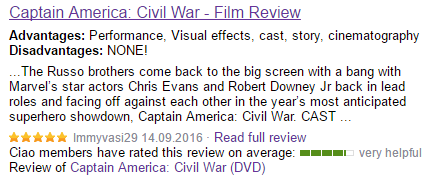
\includegraphics[width=\linewidth]{figure/item_review_example}
        \caption{An item review example}
        \label{item_review_example}
    \end{subfigure}
    \begin{subfigure}[b]{0.35\textwidth}
        \centering
        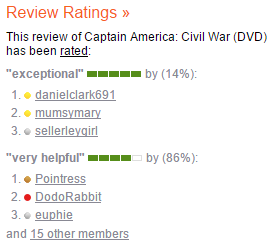
\includegraphics[width=\linewidth]{figure/helpfulness_rating_example}
        \caption{A helpfulness rating example}
        \label{helpfulness_rating_example}
    \end{subfigure}
    \caption{Item review and helpfulness rating example from Ciao}
    \label{real_world_example}
\end{figure}

Wang et al. \cite{DualRole} considered helpfulness rating as users’ implicit feedback about items, and  incorporated the helpfulness rater role in recommendation systems to mitigate data sparsity and cold-start problems.
Raghavan et al. \cite{RQMF} proposed collaborative filtering that considers quality of review to improve performance in the presence of fake reviews.
% With the assumption that spurious reviews would get negative helpfulness ratings, they measure the quality of a review by aggregating the helpfulness ratings about the review, and lower the impact of low-quality reviews on optimizing parameters of recommendation model.
Assuming that fake reviews receive a negative helpfulness rating, the proposed model measures the quality of a review by aggregating the helpfulness ratings for the review, and lowers the impact of poor quality reviews on optimizing parameters of recommendation model.
They show that incorporating review helpfulness rating information has potential benefits of improving the performance and robustness of recommendation systems.

% However, these studies do not deal with manipulating review helpfulness attack.
However, they did not deal with fake review helpfulness ratings.
After injecting fake reviews, malicious attackers can easily inject fake helpfulness ratings to promote the quality of fake reviews.
They did not consider review quality manipulations that can promote the negative effect of fake reviews.

We propose a robust recommendation model even in the presence of both fake reviews and helpfulness ratings via a new review quality measure which estimates the true quality of reviews.
Our approach consists of three stages.
The first stage involves mapping users to a feature vector space to find groups of users suspected of being shillers.
In the second stage, the quality of each review is measured based on the Bayesian weighted mean of the helpfulness ratings associated with each review.
If a helpfulness rater is suspicious, that is, he/she is very similar to a review writer, his/her helpfulness rating should have a low weight.
In the final stage, the quality of each review measured in the previous stage is used as input for collaborative filtering.
We adopt the cost function suggested by \cite{ImplicitCF,RQMF}.
Simulating various attacks on a real-world dataset, we demonstrate the effectiveness of the proposed method
We show that our method mitigates the effect of manipulating review quality compared with other methods.
In specific, our method yields up to 20 times more robust recommendation results than the approaches that do not consider attacks.
%The first stage involves the task of mapping users to a feature vector space such that users who are similar in terms of behaviors related to shilling attacks are located in close proximity to one another in the space.
%In the second stage, the quality of each review is measured by the Bayesian weighted mean of the helpfulness ratings associated with each review.
%A helpfulness rating is “down-weighted” if the similarity between the feature vectors of the helpfulness rater and the writer of the associated review is above the predetermined threshold.
%In the final stage, the quality of each review measured in the previous stage is used to collaborative filtering.
%We adopt the cost function suggested by \cite{RQMF,ImplicitCF}.
%We demonstrate the effectiveness of the proposed method by measuring the effect of various attacks on a real-world dataset.
%Compared with other methods, proposed method mitigates the effect of manipulating review helpfulness.

The thesis is organized as follows.
Chapter 2 presents the background.
Related work is described in Chapter 3.
Our problem is defined in Chapter 4 and Chapter 5 describe our approach.
In Chapter 6 presents the experimental methodology used to evaluate the robustness of our approach and results of our experiment.
Finally, we conclude in Chapter 7.



%%
%% 그림 삽입 예시
%% Example. how to insert graph
%%
%% Note. 가급적 \includegraphics 명령을 사용하십시오.
%% Recommen : Use \includegraphics to insert graph.
%%
%\begin{figure}
%    \centering
%    \subfigure[An item review example]
%    {
%        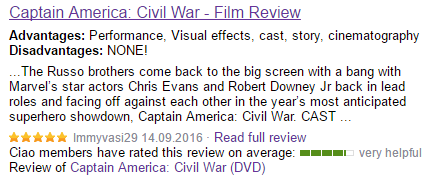
\includegraphics[width=9cm]{figure/item_review_example}
%        \label{item_review_example}
%    }
%    \subfigure[A helpfulness rating example]
%    {
%        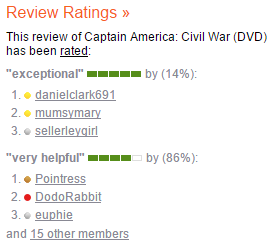
\includegraphics[width=4cm]{figure/helpfulness_rating_example}
%        \label{helpfulness_rating_example}
%    }
%    \caption{Item review and helpfulness rating example from Ciao}
%    \label{real_world_example}
%\end{figure}





%\begin{figure}[h]
%    \centerline{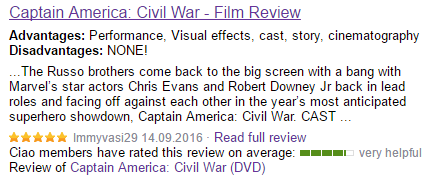
\includegraphics[width=7.5cm]{figure/item_review_example}}
%    \caption{ An item review example    } \label{item_review_example}
%\end{figure}
%
%\begin{figure}[h]
%    \centerline{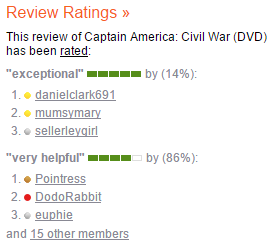
\includegraphics[width=5.5cm]{figure/helpfulness_rating_example}}
%    \caption{ A helpfulness rating example    } \label{helpfulness_rating_example}
%\end{figure}

\chapter{Background}
\section{Notation}
Throughout the thesis, sets are denoted as italic capital letters and matrices/tensors are written as boldface capital letters.
Let $U = \{u_1,u_2,…,u_n\}$ and $I = \{i_1,i_2,…,i_m\}$ be a set of users and items where $n$ and $m$ are the number of users and items, respectively.
In recommendation systems, users can rate items in the form of a numeric rating score accompanied by review text.
We use the term \textit{'item rating'} and \textit{'review'} to represent a numeric rating score for an item.
%We use the term 'review' to represent both numeric rating and review text.
%Unless otherwise mentioned, the term ‘review’ of a user for an item indicates numeric rating the user give to the item.
We use the matrix $ \bm{R} \in \mathbb{R}^{n \times m} $ to denote the item rating matrix where an entry $ R_{u,i} $ indicates the item rating score of user $u$ for item $i$.
Note that the item rating matrix $\bm{R}$ is sparse since users usually rate a small set of items.
If user $u$ did not rate item $i$, then we assign “?” to the missing item rating $\bm{R}_{u,i}$.
$IR=\{(u,i,ir)| u \in U,i \in I,ir=\bm{R}_{u,i},ir \neq ? \}$ to represents item rating dataset where $(u,i,ir)$ means user $u$ rates item $i$ with score $ir$.

Many recommendation systems allow users to evaluate the helpfulness of other users’ reviews in order to improve the user experience.
After reading review content (numeric rating score and review text), users give the review helpfulness score in the form of a numeric rating score.
We use the term \textit{'helpfulness rating'} to indicate such a numeric rating score for a review.
$(u_a,u_b,i_c,hr)$ means that user $u_a$ gives helpfulness score $hr$ to the review of user $u_b$ for item $i_c$.
We use $\bm{H} \in \mathbb{R}^{n \times n \times m}$ to denote the helpfulness rating tensor where an entry $\bm{H}_{a,b,c}$ indicates the review helpfulness score that user $a$ gives to the review of user $b$ for item $c$.
Similarly with item rating dataset, $HR=\{(u_a,u_b,i,hr)| u_a,u_b \in U,i \in I,hr=\bm{H}_{a,b,c},hr \neq ?\}$ represents helpfulness rating dataset.

Since we consider an attacker who injects shillers, we use $U^g$ and $U^f$ to denote the set of genuine users and shillers, respectively.
Genuine item rating and helpfulness rating dataset are denoted by $IR^g=\{(u,i,ir)|u \in U^g\}$ and $HR^g=\{(u,v,i,hr)|u \in U^g\}$, respectively.
Similarly, fake item rating and helpfulness rating dataset are denoted by $IR^f=\{(u,i,ir)|u \in U^f\}$ and $HR^f=\{(u,v,i,hr)|u \in U^f\}$, respectively.
%the maximum rating on the rating scale.
Unless otherwise noted, the range of item rating score is from 1 to 5, and helpfulness rating score ranges from 0 to 5.

\section{Matrix Factorization Based Collaborative Filtering}
\begin{figure}[b]
    \centering
    \begin{subfigure}[b]{0.45\textwidth}
        \centering
        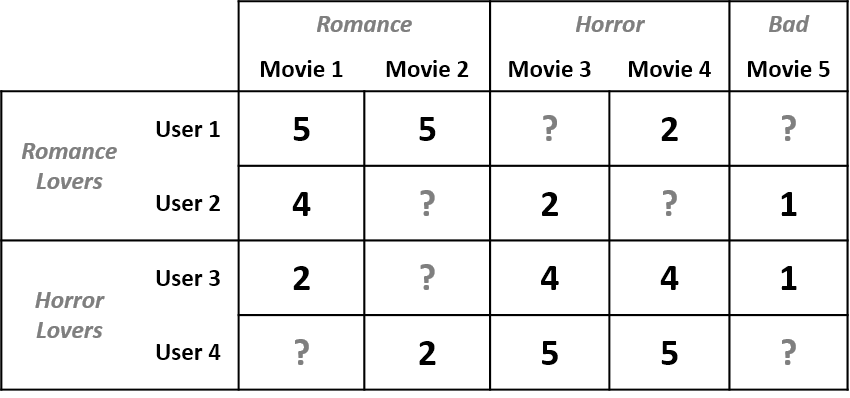
\includegraphics[width=\textwidth]{figure/mf_before_rating}
        \caption{Rating matrix $\bm{R}$}
        \label{mf_before_rating}
    \end{subfigure}
    \begin{subfigure}[b]{0.45\textwidth}
        \centering
        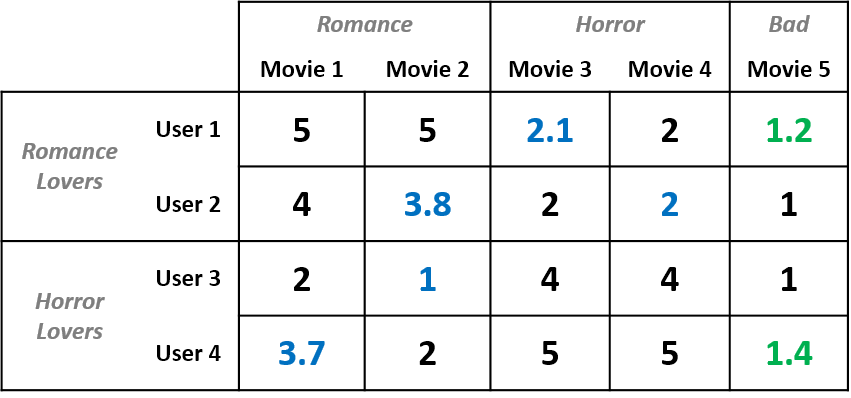
\includegraphics[width=\textwidth]{figure/mf_before_prediction}
        \caption{Prediction matrix $\bm{UV}$}
        \label{mf_before_prediction}
    \end{subfigure}
    \caption{Matrix factorization example}
    \label{mf_base}
\end{figure}
The objective of collaborative filtering (CF) is to predict the value of the missing entries in a item rating matrix.
Matrix factorization (MF) is the popular technique to predict the missing entries in a matrix by inferring latent patterns from the observed entries of the matrix.
In the context of CF, MF infers latent features of user and items based on the known item ratings of users for items.
It decomposes a item rating matrix $\bm{R}$ into two latent matrices $\bm{U} \in \mathbb{R}^{n \times d}$ and $\bm{V} \in \mathbb{R}^{d \times m}$ corresponding latent features of user and item, respectively, where the $d$ is the number of latent features.
In specific, MF optimizes the two matrices $\bm{U}$ and $\bm{V}$ by minimizing the following cost function which is the sum of prediction error terms and regularization terms.
\begin{equation}
Cost(\bm{U},\bm{V} | \bm{R})=\sum_{\bm{R}_{i,j} \neq ?} (  \bm{R}_{i,j} - (\bm{UV})_{i,j} )^2 + \lambda(||\bm{U}||_F^2+||\bm{V}||_F^2)
\end{equation}
After obtaining the optimized $\bm{U}$ and $\bm{V}$, all missing entries in the item rating matrix $\bm{R}$ are predicted via the dense matrix $\bm{UV}$ which is the product of $\bm{U}$ and $\bm{V}$.
% The figure \ref{mf_base} indicates a toy example of MF.
% Observed rating matrix (Figure \ref{mf_base} ) represents user-movie rating matrix.
We construct a very simple example (Figure \ref{mf_base}) as follows.
The item set of the item rating matrix consists of two romance movies, two horror movies, and one bad movie.
The user set of the item rating matrix consists of two romance lovers and two horror lovers.
After performing MF on the item rating matrix $\bm{R}$, prediction matrix $\bm{UV}$ captures the tastes of users and judges that users would not like the bad movie.


\section{Shilling Attack}
\begin{figure}[b]
    \centering
    \begin{subfigure}[b]{0.45\textwidth}
        \centering
        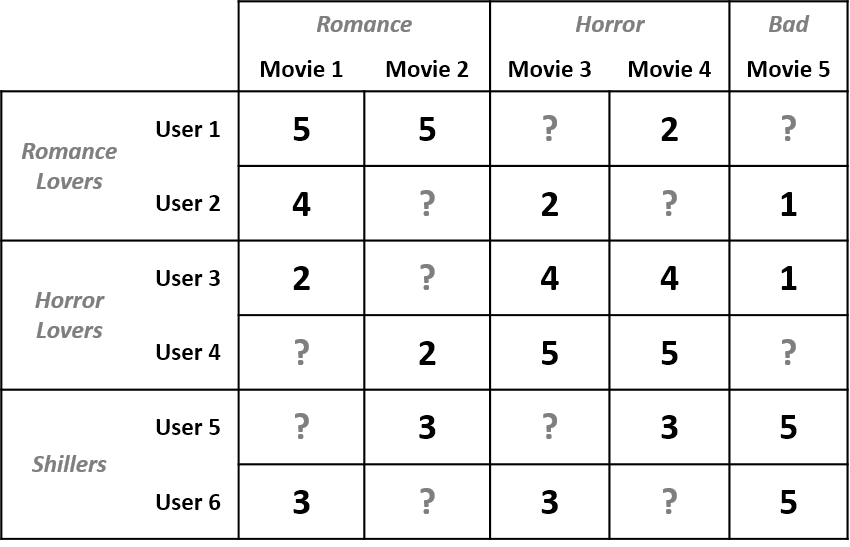
\includegraphics[width=\textwidth]{figure/mf_after_rating}
        \caption{Rating matrix $\bm{R}$}
        \label{mf_after_rating}
    \end{subfigure}
    \begin{subfigure}[b]{0.45\textwidth}
        \centering
        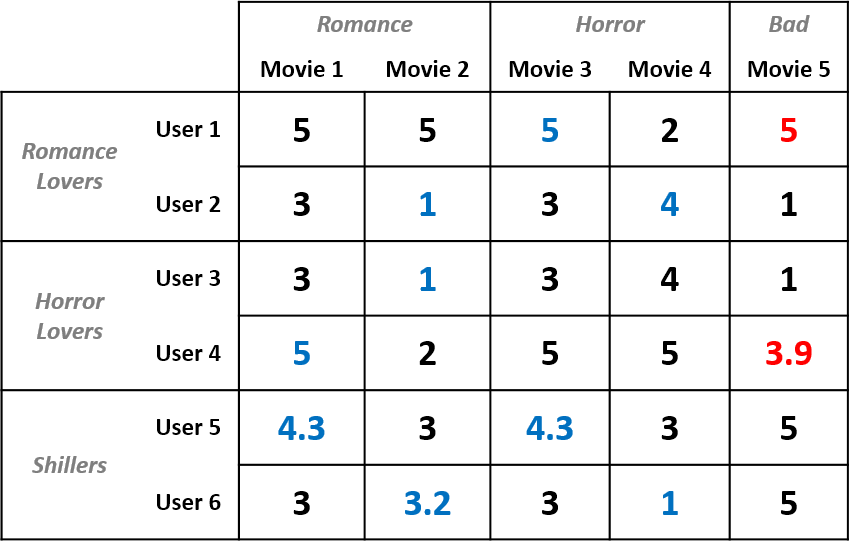
\includegraphics[width=\textwidth]{figure/mf_after_prediction}
        \caption{Prediction matrix $\bm{UV}$}
        \label{mf_after_prediction}
    \end{subfigure}
    \caption{Matrix factorization in the presence of shilling attack}
    \label{mf_attacked}
\end{figure}
There are malicious attackers who try to manipulate a CF-based recommendation system to gain benefit.
These attackers attempt to manipulate the recommendation system by injecting fraudulent user (Shillers) and fake rating data.
The attempts are called 'Shilling attacks.'
Shilling attacks are divided into two categories: \textit{push attack} and \textit{nuke attack}.
% \textit{push attacks} inject shillers which give high item ratings to particular items to promote the recommendation score for the particular items, while \textit{nuke attacks} inject shillers which give low item ratings to particular items aiming at decreasing the popularity of the items.
The push attack generates shillers with high ratings on an item to promote its recommendation score.
While the nuke attack inject shillers with low ratings on an item to decrease its popularity.
%The goal of Shilling attacks is to manipulate the recommendation results for the particular items for other genuine users.
However, fake item rating injection associated with target items only is not enough to manipulate a CF-based recommendation system, because CF predicts missing item ratings of genuine users in the way attackers wish if tastes of genuine users are similar to those of shillers.
% Collaborative filtering recommends genuine users to the direction shilling attacks wish if it recognizes that genuine users are similar to shillers.
In order to fully exploit the principle of collaborative filtering, shillers have to mimic rating behaviors of genuine users.
There are various attack models on how to mimic rating behavior of genuine users: Random attack, Average attack, Bandwagon attack \cite{shilling_attack_1,shilling_attack_2,shilling_attack_3,shilling_attack_guide}.
%[Burke et al. 2006].
In the context of push attack, Random attack injects shillers who give the highest rating to their target items and rate the randomly chosen items around the overall mean.
Average attack generates shillers that give the highest rating to their target items and the mean rating of each item to randomly chosen items.
Bandwagon attack consists of shillers whose ratings for their target items and popular items are maximum.

The figure \ref{mf_attacked} shows an example of shilling attack and its effect. We inject two shillers whose aims are boosting the prediction score of the bad movie.
Shillers rate the bad movie with the highest possible rating value, i.e. 5, and rate other movies in a similar way to other genuine users.
Matrix factoring misjudges the prediction scores of the bad movie because it has to reduce the error of the fake ratings to optimize its cost function.
Compared with figure \ref{mf_base}, figure \ref{mf_attacked} contains high predicted rating of genuine users for the bad movie.


\section{Weighted Matrix Factorization for Robust Collaborative Filtering}
The reason MF is vulnerable to shilling attack is that MF does not consider the presence of fake item ratings.
Therefore, various attempts have been proposed to eliminate or mitigate the impact of fake item ratings on MF.
The cost functions used in these attempts are expressed in the form of weighted matrix factorization(WMF) \cite{ImplicitCF}.
\begin{equation}
Cost(\bm{U},\bm{V} | \bm{W}, \bm{R})=\sum_{\bm{R}_{u,i} \neq ?} \bm{W}_{u,i}(  \bm{R}_{u,i} - (\bm{UV})_{u,i} )^2 + \lambda(||\bm{U}||_F^2+||\bm{V}||_F^2)
\end{equation}
$\bm{W} \in \mathbb{R}^{n \times m}$ is a weight matrix where $\bm{W}_{u,i}$ is the weight for the item rating $\bm{R}_{u,i}$.
In this cost function, prediction error term changes from sum of squared errors to weighted sum of squared errors, which allows item ratings whose weight is small to have significant prediction error.
This property helps WMF based on weight matrix where fake item ratings have a small weight to yield desirable predictions robust to fake item ratings.

Figure \ref{wmf_good} shows an example of WMF where the weights of genuine reviews are larger than those of fake reviews.
With well-assigned weight matrix, latent features of users and items are optimized to describe genuine review better, so shillers fail to manipulate prediction of genuine users for the bad movie.

\begin{figure}[h]
    \centering
    \begin{subfigure}[b]{0.3\textwidth}
        \centering
        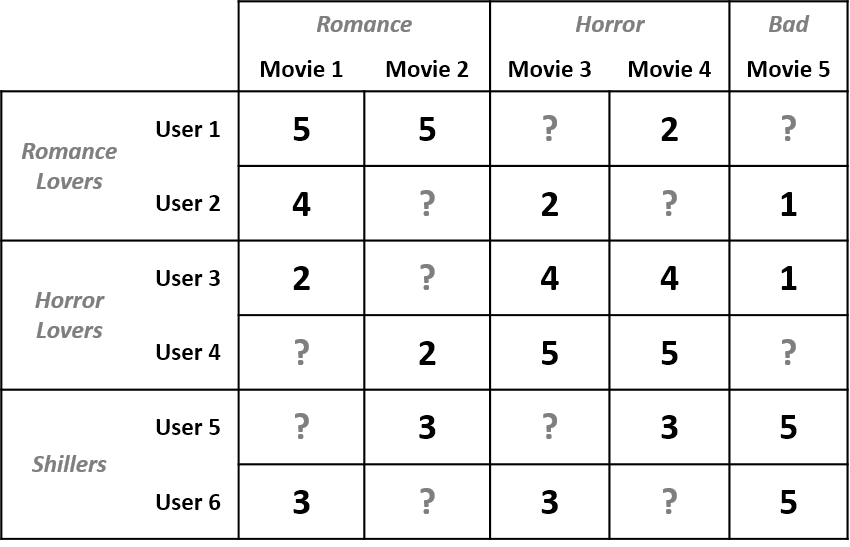
\includegraphics[width=\textwidth]{figure/mf_after_rating}
        \caption{Rating matrix $\bm{R}$}
        %\label{mf_after_rating}
    \end{subfigure}
    \begin{subfigure}[b]{0.3\textwidth}
        \centering
        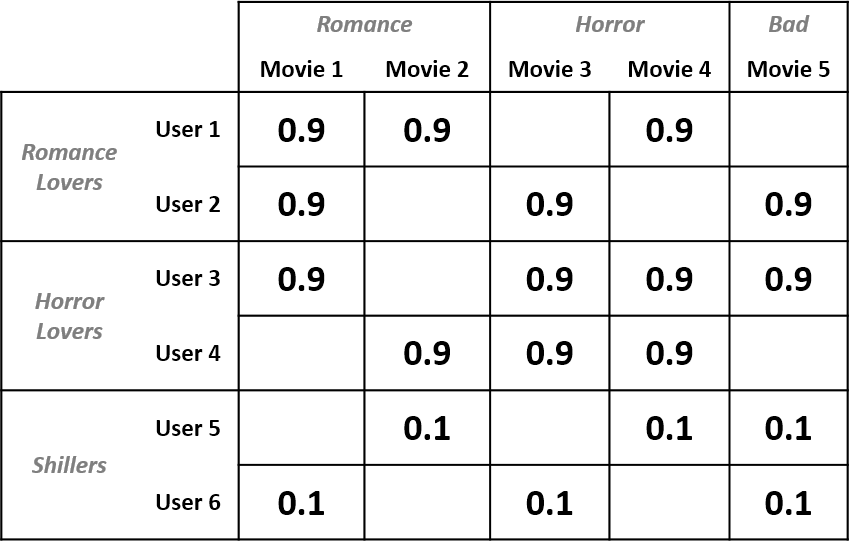
\includegraphics[width=\textwidth]{figure/wmf_good_weight}
        \caption{Weight matrix $\bm{W}$}
        \label{wmf_good_weight}
    \end{subfigure}
    \begin{subfigure}[b]{0.3\textwidth}
        \centering
        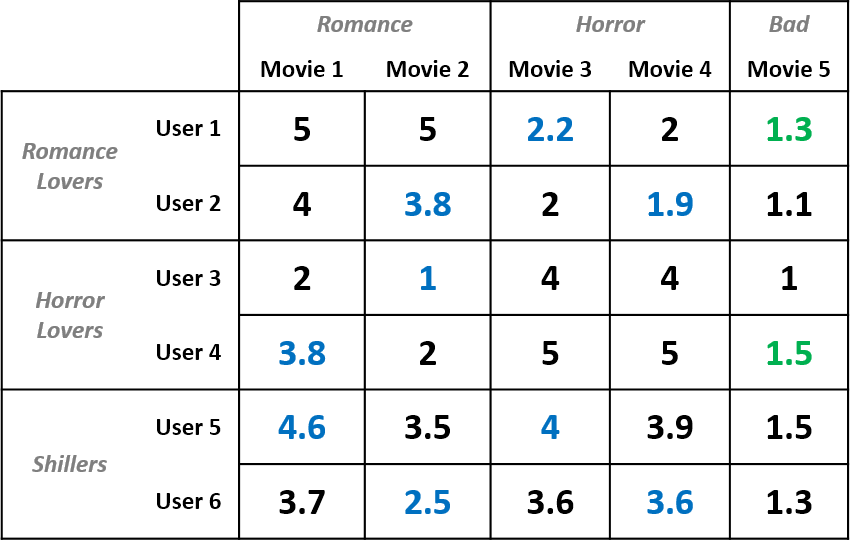
\includegraphics[width=\textwidth]{figure/wmf_good_prediction}
        \caption{Prediction matrix $\bm{UV}$}
        \label{wmf_good_prediction}
    \end{subfigure}
    \caption{Weighted matrix factorization with a well assigned weight matrix}
    \label{wmf_good}
\end{figure}


However, if the weights of fake item ratings are large, then WMF would yield more manipulated predictions.
Therefore, the key to WMF for robust CF is how to build a good weight matrix $\bm{W}$, in other words, how to capture fake item ratings and decrease their weights.


%They use the following cost function proposed by \cite{ImplicitCF} to treat the helpfulness of a review as the weight of the review.
%\begin{equation}
%Cost(\bm{U},\bm{V} | \bm{W} \bm{R})=\sum_{\bm{R}_{i,j} \neq ?} \bm{W}_{i,j}(  \bm{R}_{i,j} - (\bm{UV})_{i,j} )^2 + \lambda(||\bm{U}||_F^2+||\bm{V}||_F^2)
%\end{equation}
%In this cost function, prediction error term changes from sum of squared errors to weighted sum of squared errors.
%In other words, this cost function measures the error of a weighted matrix factorization.
%Therefore, the weighted sum of errors allows unhelpful reviews to have a significant error but penalizes error of helpful reviews heavily.

\chapter{Related Work}
This section describes various approaches to build a weight matrix.
The common goal is to detect suspicious item ratings and assign low weight.

%Our paper is related to the following topics: robust recommendation and review helpfulness.
%We discuss the two topic in the following subsections.

%\section{Robust Recommendation}
% robust statistical model
Early research for robust CF focused on detecting manipulated ratings by only examining a given rating matrix.
For example, Mehta et al. \cite{RMF} proposed Robust Matrix Factorization (RMF) using M-estimators to bound the effect of outliers and noisy data.
\cite{LiesAndPropaganda,UnsupervisedShilling,AttackResistant} apply PCA-based variable selection to detect suspicious users in unsupervised setting.

Recently, many researchers have started to incorporate various types of additional information into the recommendation algorithm in order to improve the accuracy of the recommendation algorithm.
In response to this trend, defense mechanisms with additional information have also been proposed.
Three popular additional information used in the recommendation algorithm are review text and review helpfulness rating information.

% Fake review detection - (supervised) textual feature, meta-feature
Text-based approaches \cite{text_duplicate, text_crowd,text_opinion_summarization,naive_helpfulness} exploit review textual features and meta features to detect fake reviews.
\cite{text_duplicate} detects spam reviews by finding (near) duplicate reviews and using learned logistic regression with manually labeled data.
Ott et al. \cite{text_crowd} collected training data through crowd-sourcing and accurately classified the deceptiveness of reviews based on n-grams.
However, text-based approaches have several drawbacks.
They require labeled data to train an accurate classifier, and the labeled data depends on the item domain.

%Review Helpfulness
Many review sites adopt votes on the helpfulness of reviews.
With helpfulness ratings, users can examine the helpfulness of reviews with statistics such as “90 (out of 100) people found this review helpful” or “40 members have rated this review on average (somewhat helpful)”.
Some research \cite{naive_helpfulness,RQMF} exploit helpfulness rating information to measure the quality of reviews.
Kim et al. \cite{naive_helpfulness} proposed the measure to quantify the quality of a review by aggregating helpfulness ratings for the review.
\begin{equation} \label{eq:naive_quality}
Quality(review(u,i))=\frac{1} {N} \sum_{\bm{H}_{v,u,i} \neq ?} \bm{H}_{v,u,i}
\end{equation}
where $N$ is the number of helpfulness ratings for review (item rating) $\bm{R}_{u,i}$.
Under the assumption that spam reviews would receive low helpfulness ratings, \cite{RQMF} builds the weight matrix used in the WMF with the above review quality measure.
They show that review helpfulness could improve the overall performance of recommendation in the presence of spam review.

\chapter{Motivation}
\section{Review Quality Manipulation}
The review quality measure  represented by the equation ~\ref{eq:naive_quality} relies on the naive assumption that all helpfulness ratings are genuine.
However, this assumption is easily violated if attackers inject fake helpfulness ratings to promote the quality of their fake reviews.
From an adversarial perspective, the cost of fake helpfulness rating injection would be not much more expensive than the cost of fake item rating injection.
Therefore, when constructing weight matrix based on review helpfulness ratings, attempts to review quality manipulation should be thoroughly taken into account.

Figure \ref{wmf_bad} shows the case an attacker succeeds in manipulating the quality of fake reviews.
The fake item ratings for the bad movie have a larger weight than other genuine item ratings as shown in Figure \ref{wmf_bad}.
% Due to the manipulated weight matrix, collaborative filtering outputs prediction matrix weighted toward fake reviews.
Due to the manipulated weight matrix, the recommendation result is largely affected.

\begin{figure}[h]
    \centering
    \begin{subfigure}[b]{0.3\textwidth}
        \centering
        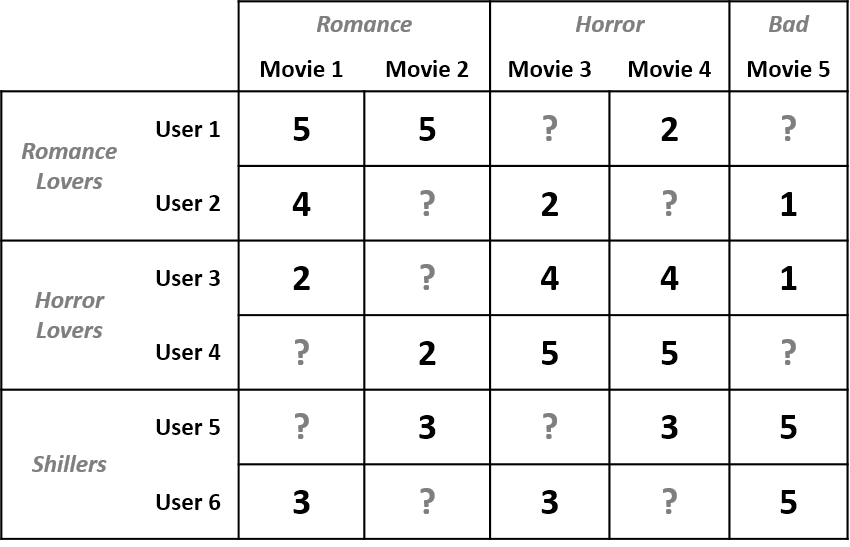
\includegraphics[width=\textwidth]{figure/mf_after_rating}
        \caption{Rating matrix $\bm{R}$}
        %\label{mf_after_rating}
    \end{subfigure}
    \begin{subfigure}[b]{0.3\textwidth}
        \centering
        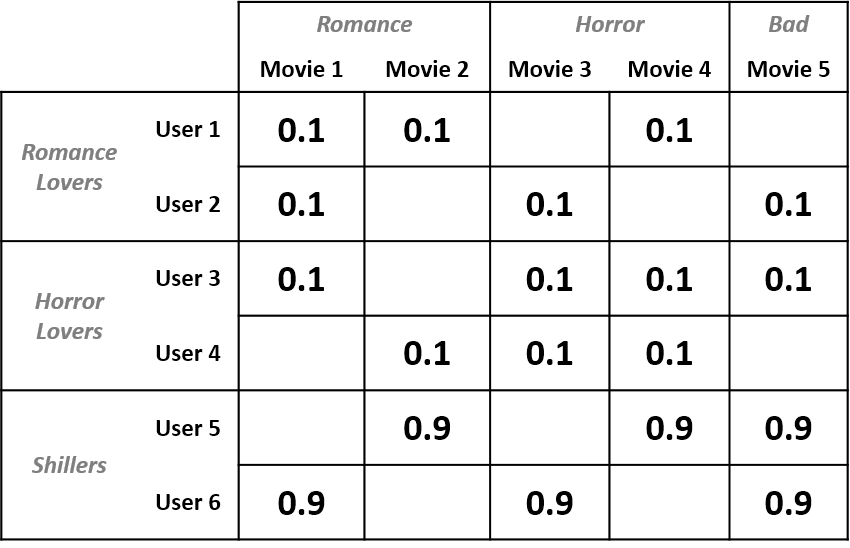
\includegraphics[width=\textwidth]{figure/wmf_bad_weight}
        \caption{Weight matrix $\bm{W}$}
        \label{wmf_bad_weight}
    \end{subfigure}
    \begin{subfigure}[b]{0.3\textwidth}
        \centering
        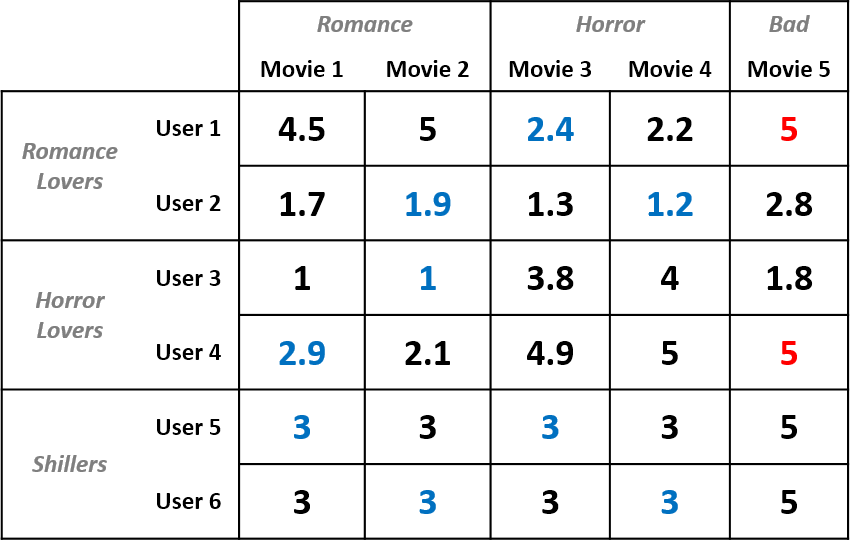
\includegraphics[width=\textwidth]{figure/wmf_bad_prediction}
        \caption{Prediction matrix $\bm{UV}$}
        \label{wmf_bad_prediction}
    \end{subfigure}
    \caption{Weighted matrix factorization with a badly assigned weight matrix}
    \label{wmf_bad}
\end{figure}


\section{Attack Model}
% // Target items are poorly rated by some genuine users.
In this section, we define an attack model.
% The objective of our attack model is to manipulate collaborative filtering, which considers review quality, to increase overall predicted ratings for the target items.
The attack model injects both fake item review rating and fake helpfulness rating in order to simulate a push attack.
We only focus on push attack, because push attack is a more direct way to promote monetary benefit than nuke attack.
We leave nuke attack for future work.
Our attack model involves in injecting fake item rating and helpfulness rating dataset, $IR^f$ and $HR^f$.

\subsection{Fake Item Rating Injection}
Our attack model injects fake item ratings (reviews) to bias predicted ratings of collaborative filtering for the target items.
Popular strategies for fake item rating injection are Random attack, Average attack and Bandwagon attack.
Since Random attack is known to be ineffective, we focus on Average attack, and Bandwagon attack.
%[KDD 06]
%Attackers usually realize shilling attacks by injecting an attack profile as shown in Fig. 1, which is first defined by Bhaumik et al. (2006), Mobasher et al. (2007a) to mislead the CF system. Such profiles can be defined as four set of items (Bhaumik et al. 2006; Mobasher et al. 2007a). [from Shilling attacks against recommender systems: a comprehensive survey]
Similar to \cite{shilling_attack_guide}, from the view of each shiller, the item set $I$ is partitioned into 4 subsets, $I^{target},I^{popular},I^{filler}$  and $I^{none}$ where $I^{target}$ is a set of target items; $I^{popular}$ is a set of popular items that many genuine users like; $I^{filler}$ is a set of randomly chosen items, called filler items; and $I^{none}$ is the set of the remaining items, i.e. $I^{none}=I-I^{target}-I^{popular}-I^{filler}$.
% Each shiller rates items of $I^{target},I^{popular}$ and $I^{filler}$ as follows.
% First, each shiller rates all target items with the highest possible rating score.
% Secondly, with the aim of being similar to other users, each shiller rates each filler item of $I^{filler}$ and its rating score is the average of all ratings given to the filler item.
% Finally, to increase the probability of being similar to a large number of other users, each shiller gives the highest possible rating score for all items of $I^{popular}$.
For each shillers, item ratings for $I_{target}$, $I_{popular}$ and $I_{filler}$ are assigned as follows:
First, we assign the highest possible value to the item rating scores of shillers for $I_{target}$
Secondly, to make the rating behavior of shillers similar to that of genuine users, the item rating scores for $I_{filler}$ are distributed around the average item rating for filler items.
Finally, we let shillers give the highest item rating scores for $I_{popular}$ to increase similarity between shillers and a large number of genuine users.
%%%%%%%%%%%%%%%%%%%%
Note that the size of each subset can vary.
We assume a recommendation system manager could easily detect attacks associated with the too big size of $I_{target}$, $I_{filler}$, $I_{popular}$.
Therefore, we limit the size of each subset to less than 1\% of the size of an entire item set $I$.
In summary, general form of fake item rating dataset $IR^f$ is defined as follows.
\begin{equation}
{IR}^f = \bigcup_{u^f \in U^f} \{(u^f,i,ir_{max}) | i \in I^{target} \} \cup \{(u^f,i,ir_{avg} {(i)}) | i \in I^{filler} \} \cup \{(u^f,i,ir_{max}) | i \in I^{popular} \}
\end{equation}
$ir_{max}$ is the highest value on the item rating scale and $ir_{avg} {(i)}$ is the average item rating for item $i$.

\subsection{Fake Helpfulness Rating Injection}
% Our attack model attempts to manipulate collaborative filtering considering review quality by injecting fake helpfulness ratings for review quality manipulation.
In addition to fake item rating injection, our attack model injects fake helpfulness ratings to manipulate review quality.
The injection makes our study different from existing attack models.
%%%%
%%%%%%%% version 1
% Each shiller gives the highest helpfulness rating to all the fake reviews about target items.
% Additionally, each shiller generates random helpfulness ratings for normal reviews to avoid attack detections.
%%%%%%%%%%% comment
% The helpfulness rating of fake users is assigned to the highest value of target items.
% Additionally, the helpfulness rating of fake users is randomly generated for normal reviews to avoid attack detections
%%%%%%%%%% version 2
We set shiller's helpfulness ratings for fake reviews to the highest value.
Additionally, we inject random helpfulness rating of shillers for randomly chosen reviews aimed at avoiding attack detections
%%%%%%%%
% We call such helpfulness ratings as camouflage helpfulness ratings.
%We restrict the size of camouflage helpfulness ratings a shiller makes to less than the size of the helpfulness ratings the shillers makes.
Formally, fake helpfulness rating dataset $HR^f$ is defined as follows:
\begin{equation}
HR^f = \bigcup_{u^f \in U^f} \{(u^f,v, i, hr_{max}) | v \in U^f,i \in I^{target} \} \cup \{(u^f,v,i,hr_{random}) | v \in U^g, i \in I, \bm{R}_{v,i} \neq ? \}
\end{equation}
$hr_{max}$ is the highest value on the helpfulness rating scale and $hr_{random}$ represents random rating.

In the presence of fake helpfulness ratings, computing the quality of a review as the average of helpfulness ratings misjudges fake reviews as high quality, which increases the negative impact of fake reviews on collaborative filtering considering review quality.

\section{Problem Definition}
With the proposed attack model, we define our problem as follows: given reviews and helpfulness ratings in the presence of fake data injected by the attack model, estimate the true quality of reviews to construct the weight matrix of WMF.
We express our problem as follows.
\begin{equation} \label{eq:quality_measure}
Quality(review(u,i))=F(Helpfulness\ ratings\ of\ review(u,i)\ under\ attack)
\end{equation}
Then the problem can be divided into two sub-problems.
One is to detect fake helpfulness ratings, and the other is to devise a robust estimator $F$ that produces consistent review quality regardless of the presence of fake helpfulness ratings.


\chapter{Proposed Method}
This section describes our method in detail.
The following sections describe how to capture suspicious helpfulness ratings and how to estimate the true quality of reviews.

\section{User2Vec}
% feature learning !!!
% Word2Vec takes a text corpus as its training data and learns a mapping of words to a vector space such that words that frequently appear together in sentences have similar vectors.
Recently, various prediction tasks \cite{Word2Vec,NegativeSampling,DeepWalk,Node2Vec} have improved performance by learning the desirable features themselves, instead of manually determining domain-specific features.
Skip-gram model \cite{Word2Vec} is a popular model proposed for natural language processing task by Mikolov et al.
The goal of the Skip-gram model is to capture semantic relationships between words.
With the hypothesis that words which frequently appear together in sentences have semantic relationships, the Skip-gram model takes large real-world text corpus as training data and learns feature representations for words.
In specific, it maps words to a feature space such that words frequently appear together in sentences have similar feature vectors.
The Skip-gram model is widely adopted due to the efficiency and ability to capture useful relationships in the text data.
% example ) feature learning for network
Inspired by the success of the Skip-gram model, some researchers apply the Skip-gram model to learning a mapping of vertices of a network to vectors which encode social relation \cite{DeepWalk,Node2Vec}.
With the assumption random walk traces contain social relation between vertices, they generate samples of random walk traces as sequences of vertices, feed them into the Skip-gram model.

% analogy between
In this thesis, we propose User2Vec, an algorithm for learning feature representations for users in recommendation system to detect suspicious relationships between users.
\cite{Word2Vec} uses real-world sentences as sequences of semantically related words.
\cite{DeepWalk,Node2Vec} generates random walk traces as sequences of socially related vertices to obtain useful features for various prediction tasks.
Similar to such approaches, we generate user pairs which might contribute shilling attacks and feed them into the Skip-gram model to obtain feature representations of users which are useful to detect shillers.

To generate sequences of attack-related users, we focus on behaviors of shillers.
Several studies \cite{LiesAndPropaganda,UnsupervisedShilling} reported that shillers need to work together to maximize the effect of their attack.
This strategy is referred to as group attack.
In our attack model, shillers equally give the highest item rating to target items and the highest helpfulness rating to their fake reviews.
Taking this into consideration, we regard following relationships between users as clues to the group attack.
\begin{enumerate}
\item Both user X and Y give $ir_{max}$ for an item
\item Both user X and Y give $hr_{max}$ for a review
\item User X gives $hr_{max}$ for a review written by user Y
\end{enumerate}
We refer to the users rate an item with $ir_{max}$ as \textit{enthusiasts} for the item.
Similarly, we refer to the users rate the helpfulness of a review with $hr_{max}$ as \textit{supporters} for the review.
The first (second) relationship represents the pair of enthusiasts (supporters) whose opinions about some item (review) are same.
If user $u_c$ and $u_d$ always rate in the same way items or reviews, then it is reasonable to suspect that $u_c$ and $u_d$ are performing group attack.
The last relationship indicates the pair of a reviewer and a supporter.
If user $u_a$ always gives the maximum helpfulness rating to all reviews written by another user $u_b$, then one can doubt that user $u_a$ intentionally promotes the influence of user $u_b$.
Note that we only target the ratings with the highest score only since we focus on push attacks.
Of course, pairs of genuine users could reveal clues to the group attack due to the coincidence of opinions about items or reviews.
However, all shillers have to involve in many connections through the relationships associated with group attack as a necessity to maximize the degree of manipulation.
With this in mind, we suspect the truthfulness of a helpfulness rating if the rater and the reviewer are frequently connected through the mentioned relationships.
% Hence, we hypothesize that the users created from group attacks will frequently be connected through the following relationships.

% In this paper, aimed at learning a mapping users to vector space such that shillers injected by group attack have similar vectors,
User2Vec consists of two steps.
In the first step, we sample user pairs that reveal clues to the group attack.
Sampling user pairs corresponding to the first relationship proceeds as follows.
Among the items having at least two enthusiasts, we first sample an item with the probability proportional to the cardinality of the users associated with the item and choose two reviewers for the sampled item uniformly at random.
Sampling user pairs corresponding to both the second and last relationship involves in sampling reviews.
% For a review to be sampled, it should receive at least one supporter.
The probability of sampling a review is proportional to the number of the helpfulness raters for the review.
With a sampled review, we choose two supporters to get the sample related to the second relationship.
To generate sample correspoing to the last relaionship, we sample one supporter and produce a pair of reviewer and supporter.
In the last step, we feed the sampled user pairs into the Skip-gram model and obtain feature vectors of users.
We expect the obtained feature vectors encode group attack patterns.
In other words, shillers are very closely located to each other in the feature space, while genuine users are scattered.
Note that User2Vec, which places the shillers very close to each other in the feature space, does not guarantee that genuine users are positioned away from each other in the feature space.
However, if the dimension of the feature space is moderately high, the probability that the location of two arbitrarily selected users is close is very small.
Therefore, although there is a risk of judging false positives, we judge that the relationship between two users with very high similarity is not trustful and define the suspiciousness of a helpfulness rating as a function of the similarity between the feature vectors of the helpfulness rater and the reviewer.

\begin{algorithm}[h]
\caption{User2Vec algorithm}
\label{alg:userembedding}
\begin{algorithmic}
\Function{User2Vec} {dimensions $d$, num\_samples $n$, item rating matrix $\bm{R}$, helpfulness rating tensor $\bm{H}$}
\State Initialize $clues$ to $empty$
\For {$iter = 1$ to $n$}
    \State append EnthusiastPair($\bm{R}$) to $clues$
    \State append SupporterPair($\bm{H}$) to $clues$
    \State append ReviewerSupporterPair($\bm{H}$) to $clues$
\EndFor
\State $userVec =$ Skip-Gram($clues, d$)
\State \Return $userVec$
\EndFunction

\Function{EnthusiastPair} {item rating matrix $\bm{R}$}
    \State let $Enthusiast(item)$ be $\{u | \bm{R}_{u,item}=ir_{max}\}$
    \State let $EI$ be $\{item | |Enthusiast(item)| \geq 2 \}$
    \State sample item $i$ from $EI$ with the prob. proportional to the cardinality of $Enthusiast(i)$
    \State sample user $u,v$ from $Enthusiast(i)$ uniformly at random
    \State \Return $(u,v)$
\EndFunction

\Function{SupporterPair} {helpfulness rating tensor $\bm{H}$}
    \State let $Supporter(u,i)$ be $\{v | \bm{H}_{v,u,i}=hr_{max}\}$
    \State let $SU$ be $\{(u,i) | |Supporter(u,i)| \geq 2\}$
    \State sample review $(u,i)$ from $SU$ with the prob. proportional to the cardinality of $Supporter(u,i)$
    \State sample user $u_a,u_b$ from $Supporter(u,i)$ uniformly at random
    \State \Return $(u_a,u_b)$
\EndFunction

\Function{ReviewerSupporterPair} {helpfulness rating tensor $\bm{H}$}
    \State let $Supporter(u,i)$ be $\{v | \bm{H}_{v,u,i}=hr_{max}\}$
    \State let $SU$ be $\{(u,i)| |Supporter(u,i)| \geq 1\}$
    \State sample review $(u,i)$ from $SU$ with the prob. proportional to the cardinality of $Supporter(u,i)$
    \State sample user $v$ from $Supporter(u,i)$ uniformly at random
    \State \Return $(u,v)$
\EndFunction

% \Function{CallA}{$a$} \funclabel{alg:a} \label{alg:a-line}
%     \State \Call{CalcSquare}{$a$}
% \EndFunction
% \Statex
% \Function{CalcSquare}{$b$} \funclabel{alg:b}
%     \State \Return $b\times b$
% \EndFunction

\end{algorithmic}
\end{algorithm}


\section{Robust Review Quality Measure}
We assume that the true quality of a review can be estimated by the mean of genuine helpfulness ratings.
However, in the presence of fake helpfulness ratings, we need to estimate the true quality of a review by the weighted mean of helpfulness ratings where the fake helpfulness ratings have very low weight.
If the number of helpfulness ratings is sufficiently high, then this estimation get high confidence.
However, for reviews with have few helpfulness ratings or only fake helpfulness ratings, the weighted mean is not a robust estimator for such reviews.
Say a fake review which has only fake helpfulness ratings.
Then the output of weighted mean is biased toward fake helpfulness ratings even if the weight of fake helpfulness ratings is almost zero.
With all of these things in mind, we define the following review quality measure to estimate the true quality of a review.
\begin{equation}
Quality(u,i) = \frac{ w_{prior} Q_{default} + \sum_{v \in \{x|\bm{H}_{v,u,i} \neq ?\}} T(v,u) \times \bm{H}_{v,u,i} } {w_{prior}  + \sum_{v \in \{x|\bm{H}_{v,u,i} \neq ?\}} T(v,u) }
\end{equation}
We take Bayesian approach that incorporates both a prior belief and a weighted mean of review helpfulness ratings.
The prior quality $Q_{default}$ works as prior belief.
$w_{prior}$ is the weight given to the prior belief.
In this work, we set $Q_{default}$ as the mean of helpfulness rating range (e.g. 2.5 in the range from 0 to 5), and $w_{prior}$ as 1.
The weight of a helpfulness rating is determined by the following function $T: U \times U \rightarrow R$.
\begin{equation}
T(v,u)=
\begin{cases}
  exp(-\mu \times(cosine(userVec_v,userVec_u)-\theta)) & \text{if}\ cosine(userVec_v,userVec_u) \geq \theta \\
  1 & \text{otherwise}
\end{cases}
\end{equation}
% Armed with user2vec results, we define the suspiciousness of a helpfulness as a function of the similarity between the feature vectors of the helpfulness rater and the reviewer.
The function $T$ takes a rater and a reviewer, and output the trustfulness of the relationship between them.
$T$ penalizes the trustfulness if the cosine similarity between their feature vectors is larger than the threshold $\theta$.
As mentioned earlier, this policy might lower the weight of genuine helpfulness ratings, but the likelihood of making such a misjudgment is very low in the moderately high dimensional feature spaces.
$\mu$ is a constant for amplification of similarity.
In this work, we set the $\theta$ as 0.8 and the $\mu$ as 100.

% With the robust estimator, the quality of reviews with few helpfulness ratings will be close to the default quality $Q_{default}$, while reviews with many helpfulness ratings given by the users whose similarity to the reviewer is not that high will have a quality score close to its average helpfulness rating.
With the robust estimator, the quality of reviews with few helpfulness ratings will be close to the default quality $Q_{default}$, while reviews whose helpfulness raters are not that similar to the reviewer will have a quality score close to its average helpfulness rating.
Most importantly, reviews with many untrustful helpfulness ratings will have a helpfulness score close to the default quality $Q_{default}$.
In other words, our measure prevents fake helpfulness ratings from manipulating the quality of their fake review.

\begin{algorithm}[h!]
\caption{Robust recommendation system}
\label{alg:RRS}
\begin{algorithmic}[]

\Function{RRS} {dimensions $d$, num\_samples $n$, item rating matrix $\bm{R}$, helpfulness rating tensor $\bm{H}$}
\State $userVec = $ User2Vec($d,n,\bm{R},\bm{H}$)
\For {all review $(u,i)$}
    \State $\bm{W}_{u,i} = Quality(u,i) = \frac{ w_{prior} Q_{default} + \sum_{v \in \{x|\bm{H}_{v,u,i} \neq ?\}} T(v,u) \times \bm{H}_{v,u,i} } {w_{prior}  + \sum_{v \in \{x|\bm{H}_{v,u,i} \neq ?\}} T(v,u) }$
\EndFor
\State Optimize $Cost(\bm{U},\bm{V} | \bm{W}, \bm{R})=\sum_{\bm{R}_{i,j} \neq ?} \bm{W}_{i,j}(  \bm{R}_{i,j} - (\bm{UV})_{i,j} )^2 + \lambda(||\bm{U}||_F^2+||\bm{V}||_F^2)$

\State \Return $\bm{U}$ and $\bm{V}$

\EndFunction

\end{algorithmic}
\end{algorithm}

% Most recommendation systems for unbiasedness do not allow users to rate the helpfulness of their own reviews, i.e. “self-rating” is prohibited.
% Prohibiting self-rating can be interpreted as the effect of self-rating on recommendation system should be zero.
% Since our goal is to prevent fake helpfulness ratings from manipulating the helpfulness of fake reviews, we relax the condition of self-rating to being a very high similarity between the feature vectors of reviewer and helpfulness rater.
% Instead of zeroing the effect of self-rating, we assign the effect of modified self-rating to a small value in reverse proportion to the similarity.
% The rationale behind this choice is that very high similarity between the feature vectors of reviewer and helpfulness rater might indicate group attack and mitigating the effect of suspicious helpfulness ratings leads to unbiased helpfulness measure.
% We define the following robust helpfulness measure which estimates the true helpfulness of a review by penalizing the modified “self-rating”.

% ====================================================================================================================
% ====================================================================================================================
% ====================================================================================================================
% ====================================================================================================================

\chapter{Experiment}
\section{Experimental Setting}
We use the publicly available dataset provided by \cite{ETAF}, namely CiaoDVD.
The CiaoDVD dataset contains review and helpfulness rating information from ciao.dvd.co.uk where users rate DVDs and others’ reviews.
In the CiaoDVD dataset, users can rate items with a score from 1 to 5 as reviewer, and rate the helpfulness of reviews with a score from 0 to 5 as helpfulness rater.
From the original dataset, we filter out the reviewers who rated less than five items and items which received less than five ratings.
The statistics of the resulting dataset are shown in Table \ref{tableCiaoDVD}.
\begin{table}[h]
\caption{Statistics of CiaoDVD dataset}
\label{tableCiaoDVD}
\begin{center}
\begin{tabular} {|c|c|}
\hline
\textbf{Features} & \textbf{CiaoDVD} \\ \hline
Reviewers & 1822 \\ \hline
Items & 2069 \\ \hline
Reviews & 28374 \\ \hline
Helpfulness Rater & 27900 \\ \hline
Helpfulness Rating & 661040 \\ \hline
\end{tabular}
\end{center}
\end{table}

We assume the original data is genuine.
To this data, we inject shillers, item ratings(reviews) and helpfulness ratings as mentioned in Chapter 4.
Attack size, i.e. the number of shillers, ranges from 1\% to 3\% of total users.
Filler size is the number of $I^{filler}$ and popular size is the number of $I^{filler}$.
%Filler size + Selected size ~1\%.
We restrict the sum of filler size and popular size from exceeding 1\% of the total number of items.
We assume attacks with larger attack sizes and filler/popular sizes would be detected easily, so we decide to exclude them in our experiment setting.
% train test split
For performance evaluation, we perform 10-fold cross validation.
In each fold, the test set contains random 10\% original reviews, and the training set contains the remaining 90\% original reviews and all the fake reviews.
% target item / popular item filter,
We choose target items of $I^{target}$ as items which have been rated by at least 1\% users with below the median of the rating scale (3 in our rating scale [1,5]).
$I^{popular}$ consists of items rated items by at least 1\% users with the $ir_{max}$.
Note that $I^{filler}$ is randomly selected for each shiller.


\section{Metrics}
The objective of the experiments is two-fold. 
First, we show the proposed review quality measure has ability to estimate true quality of reviews well.
Second, we show the 
%Average helpfulness of reviews
\textbf{Average quality of reviews} measures the average quality of reviews belonging to each category.
We compare the average quality values of fake reviews and genuine reviews to find out the robustness of a quality measure.
A robust quality measure should produce the small average quality of fake reviews even in the presence of fake helpfulness ratings.

\begin{equation}
AverageHelpfulness(IR) = \frac{1}{|IR|} \sum_{ (u,i) \in IR } helpfulness(u,i)
\end{equation}
where $N_{IR}$ is the number of reviews in the $IR$.

%Prediction shift on the target items
\textbf{Prediction shift on the target items} measures the average of the change in the prediction of genuine users for the attacked items before and after a shilling attack.
In other words, this metric measures the degree of success of an attack.
The smaller the value of this metric, the more robust the recommendation method is.
\begin{equation}
PredictionShift(U,V,U',V') = \frac{1}{|U^g||I^{target}|} \sum_{u \in U^g} \sum_{i \in I^{target}} (U'V')_{u,i}-(UV)_{u,i}
\end{equation}
where $(U'V')_{u,i}$ is the predicted rating value of user $u$ for item $i$ after an attack.

\textbf{Mean Average Error(MAE) on test set} is the overall prediction error on ratings in the test set which contains 10\% of all item ratings of original users in the dataset.
MAE is commonly used to compare the predictive accuracy of recommendation algorithms.
Accurate prediction yield a small MAE.
We use MAE to measure the accuracy loss that is sacrificed to improve robustness.
\begin{equation}
MAE(U,V) = \frac{1}{|test set|} \sum_{R_{u,i} \in test set} |R_{u,i}-(UV)_{u,i}|
\end{equation}

\section{Results and Analysis}
% User2Vec result
We first visualize the results of User2Vec to show User2Vec's ability to capture shillers.
We use learned users' feature vectors as the input to the visualization tool, t-SNE \cite{TSNE}.
The users are mapped to the 2-D space.
x-shaped points represent shillers, while circle-shaped green colored points represent genuine users.
We observed that feature vectors of shillers are very close to each other.
\begin{figure}[t]
    \centerline{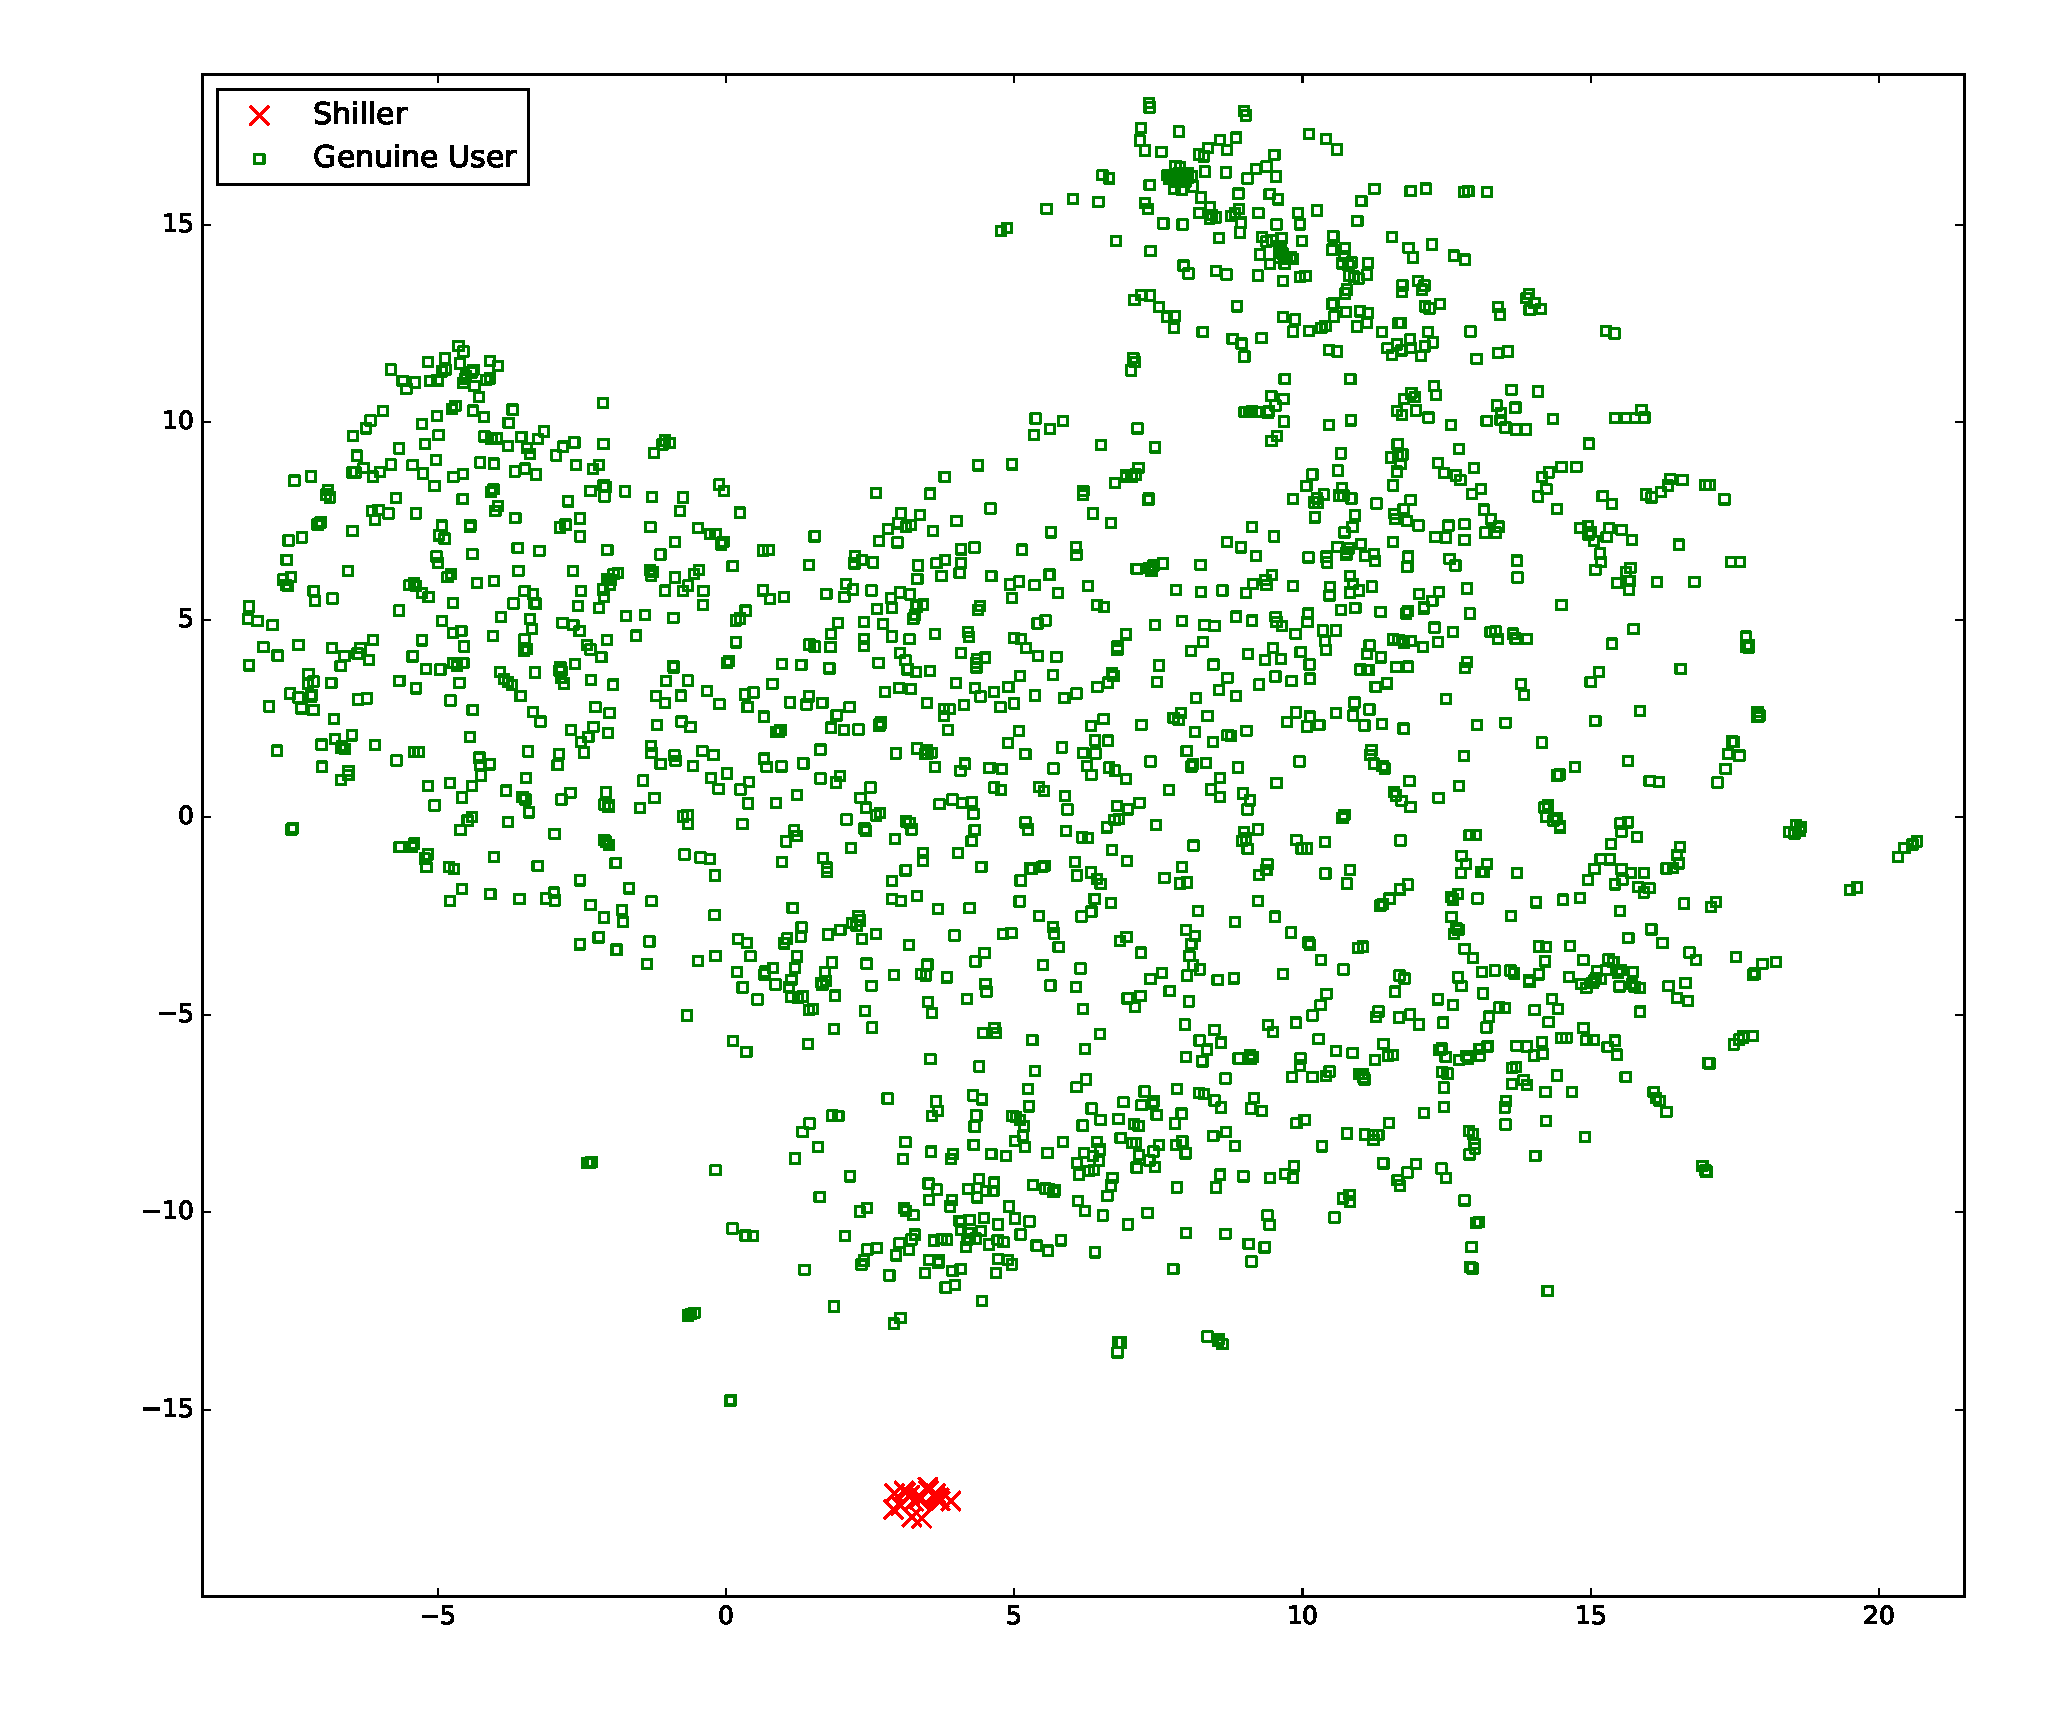
\includegraphics[width=10.5cm]{figure/user2vec_result.pdf}}
    \caption{  Visualization of the User2Vec result } \label{user2vec_result}
\end{figure}

% helpfulness measure comparison
% 1% attack size, 0.5 filler size, 0.5% popular size을 가지는 공격이 있고 차원의 크기는 32로 설정한 상황에서 우린 가짜 리뷰와 진실된 리뷰의 유용성의 평균값을 계산한다.

% we compute the average of the usefulness of fake and true reviews in the situation where fake data are injected by attacks with 1% attack size, 2% filler size, and 3% popular size. we set dimensions of user feature vectors to 32


% We first compare the average of helpfulness of fake and genuine reviews computed by each measure, varying attack size from 1\% to 3\% with fixed 0.5\% filler size, 0.5\% selected size and 32 dimensions of user feature vector.
We compute the average of the quality of fake reviews and genuine reviews.
We inject fake review through attacks with 1\% attack size, 0.5\% filler size, and 0.5\% popular size.
We set dimensions of feature vectors to 32, which is used in User2Vec.
% result explanation
As shown in table ~\ref{resultHelpfulness}, the naive quality measure results in fake reviews have a higher quality than genuine reviews, whereas our quality measure yields the opposite.
In specific, while the naive quality measure computes the quality of fake reviews at a value close to $hr_{max}$, our quality measure computes the quality of fake reviews at a value close to the default quality $Q_{default}$.
In other words, our quality measure can prevent fake helpfulness ratings from increasing the quality of fake reviews.
We observed a slight decrease in the quality of genuine reviews when using our method.
The reason for this is that the feature vector of an genuine user might be very similar to that of another genuine user by coincidence, which leads to false positive detection.
However, since the probability that false positive detection happens is very low, genuine helpfulness ratings which are wrongly sacrificed have no significant impact on estimating review quality.
Hence, our quality measure shows its ability to estimate the true quality of reviews.

% Result (helpfulness)
%----------------------- naive attack True rank 30 lda 0.0001 ---------------------
%Helpfulness distribution
%[ Fake target] Mean 1.0 [10, 25, 50, 75, 90] 1.0 1.0 1.0 1.0 1.0
%[Honest  all ] Mean 0.707772781236 [10, 25, 50, 75, 90] 0.5 0.62 0.776 0.8 0.807407407407
%[Honest target] Mean 0.752601402364 [10, 25, 50, 75, 90] 0.613846153846 0.742721164614 0.79625 0.800427350427 0.812090322581
%----------------------- robust attack True rank 30 lda 0.0001 ---------------------
%Helpfulness distribution
%[ Fake target] Mean 0.500005215262 [10, 25, 50, 75, 90] 0.500000899783 0.500001278803 0.500001819832 0.500003403991 0.500012499609
%[Honest  all ] Mean 0.690197908439 [10, 25, 50, 75, 90] 0.5 0.59375 0.750000105113 0.788920774322 0.798
%[Honest target] Mean 0.742774662194 [10, 25, 50, 75, 90] 0.60599378882 0.7359375 0.783293269231 0.793191037632 0.803526694633

\begin{table}[h]
\caption{Review helpfulness results. The range of helpfulness is from 0 to 5}
\label{resultHelpfulness}
\begin{center}
\begin{tabular}{|c|c|c|c|c|}
\hline
\multirow{2}{*}{Attack Size} & \multicolumn{2}{c|}{\begin{tabular}[c]{@{}c@{}}Naïve Helpfulness Measure\end{tabular}} & \multicolumn{2}{c|}{Our Helpfulness Measure} \\ \cline{2-5}
                             & Fake Reviews                              & Genuine Reviews                              & Fake Reviews       & Genuine Reviews       \\ \hline
%1\%                          & 4.86                                      & 3.45                                           & 2.5                & 3.45                    \\ \hline
%3\%                          & 4.95                                      & 3.45                                           & 2.5                & 3.45                    \\ \hline
1\%                          & 5.0                                      & 3.5388                                           & 2.5                & 3.45                    \\ \hline
\end{tabular}
\end{center}
\end{table}

% Prediction shift
To compare the robustness, we compute the prediction shift on the target items of algorithms using different review quality measures under attacks in the variety of attack sizes, filler sizes, and popular sizes.
From Table ~\ref{resultPredictionShift}, we observe that the WMF using our quality measure leads to the lowest prediction shift on the target items in all conditions.
The reason for this is that fake item ratings have the least impact on prediction when applying our quality measure rather than applying other methods.
Since fake helpfulness ratings increase the influence of fake item ratings on prediction when applying the naive quality measure than when ignoring review quality, the naive quality measure causes larger prediction shift on the target items than MF in the presence of fake helpfulness ratings.
Therefore we argue that our method is resistant to review quality manipulations.
% adds robustness to WMF.


%Naive review helpfulness measure를 이용한 collaborative filtering은 helpfulness를 고려하지 않은 즉, 모든 review의 중요도를 동일하게 본 baseline method보다 latent feature가 fake review의 error를 낮추는 방향으로 최적화된다. 그로 인해 공격의 영향력이 더 강화되어 더 큰 prediction shift를 보이게 된다.

\begin{table}[h]
\caption{Prediction shift on the target items}
\label{resultPredictionShift}
\begin{center}
\begin{tabular}{|c|c|c|c|c|c|}
\hline
\textbf{Attack size} & \textbf{Filler Size} & \textbf{Popular Size} & \textbf{Base} & \textbf{Naive} & \textbf{Ours} \\ \hline
\multirow{3}{*}{1\%} & 1\%                  & 0\%                   & 1.01465       & 1.7805         & \textbf{0.092686} \\ \cline{2-6}
                     & 0.50\%               & 0.50\%                & 1.48154       & 1.90081        & \textbf{0.239489} \\ \cline{2-6}
                     & 0\%                  & 1\%                   & 1.72337       & 1.79765        & \textbf{0.246163} \\ \hline
\multirow{3}{*}{2\%} & 1\%                  & 0\%                   & 1.5178        & 2.28872        & \textbf{0.172815} \\ \cline{2-6}
                     & 0.50\%               & 0.50\%                & 1.91454       & 2.30772        & \textbf{0.387328} \\ \cline{2-6}
                     & 0\%                  & 1\%                   & 2.08557       & 2.1092         & \textbf{0.469354} \\ \hline
\multirow{3}{*}{3\%} & 1\%                  & 0\%                   & 1.79902       & 2.5618         & \textbf{0.307992} \\ \cline{2-6}
                     & 0.50\%               & 0.50\%                & 1.89458       & 2.49592        & \textbf{0.580003} \\ \cline{2-6}
                     & 0\%                  & 1\%                   & 1.99723       & 2.24161        & \textbf{0.659305} \\ \hline
\end{tabular}
\end{center}
\end{table}

% MAE result (ver 1.0)
We also investigate the predictive performance of each method.
We compute MAE on the test set.
%when the training set contains fake item ratings.
According to ~\ref{resultMAE}, MF performs better than WMFs.
In fact, MAE is not ideal metric to measure the predictive performance of WMF, because MAE gives equal importance to the errors of all the ratings in the test set.
% While weighted matrix factorization tends to be fitted more toward important ratings, MAE gives equal importance to all ratings of the test set.
Even though MAE is not proper metric for WMF, MAE results of WMF are not significantly different from those of MF.
We compute Cohen's $d$ for the effect size based on means of predictive errors between MF and WMF using our quality measure.
The value of Cohen's $d$ is near 0.02, which is a small value according to \cite{EffectSize}.
Consequently, we conclude that WMF using our quality measure provides robustness at a not significant additional cost of predictive accuracy.


%추천 시스템의 본연의 목적은 사용자의 예상 평점을 맞추는 것이기 때문에 예상 평점을 맞추는 퍼포먼스를 비교한다. 공격에 의해 아무리 바뀌지 않는 방법이더라도 예상 평점의 정확도가 너무 떨어지는 방법은 바람직하지 않다.
%//예를 들면 overall mean rating(4.02314289071)로 전부 예상하면 MAE는 0.820751825687 (더 좋다….). 우리의 방법은 attack이 1\%일땐 naïve가 ours보다 좋은데 3\%일땐 그 반대가 된다. 이유는…..몰라
%performance에서 손해를 보지만 그 손해가 몇 퍼센트 차이가 나지 않는다.
%이 metric은 test dataset에 소속된 rating의 중요도를 모두 1로 보았기 때문에 review helpfulness를 고려한 추천 시스템의 퍼포먼스를 측정하기엔 완벽한 선택은 아니다. 그럼에도 불구하고 base와 그리 차이 나지 않는 performance를 보여주기 때문에 우리 방법도 괜찮다(?)


\begin{table}[h]
\caption{MAE on test set}
\label{resultMAE}
\begin{center}
\begin{tabular}{|c|c|c|c|c|c|}
\hline
\textbf{Attack Size} & \textbf{Filler Size} & \textbf{Popular Size} & \textbf{Base} & \textbf{Naive} & \textbf{Ours}     \\ \hline
\multirow{3}{*}{1\%} & 1\%                  & 0\%                   & \textbf{0.821944}      & 0.831673       & 0.843252 \\ \cline{2-6}
                     & 0.5\%               & 0.5\%                & \textbf{0.825909}      & 0.836473       & 0.842159 \\ \cline{2-6}
                     & 0\%                  & 1\%                   & \textbf{0.825078}      & 0.837706       & 0.84074  \\ \hline
\multirow{3}{*}{2\%} & 1\%                  & 0\%                   & \textbf{0.820305}      & 0.826343       & 0.840074 \\ \cline{2-6}
                     & 0.5\%               & 0.5\%                & \textbf{0.826043}      & 0.834851       & 0.836148 \\ \cline{2-6}
                     & 0\%                  & 1\%                   & \textbf{0.822775}      & 0.847235       & 0.843203 \\ \hline
\multirow{3}{*}{3\%} & 1\%                  & 0\%                   & \textbf{0.816267}      & 0.828714       & 0.840653 \\ \cline{2-6}
                     & 0.5\%               & 0.5\%                & \textbf{0.825463}      & 0.846773       & 0.841859 \\ \cline{2-6}
                     & 0\%                  & 1\%                   & \textbf{0.829685}      & 0.85275        & 0.841454 \\ \hline
\end{tabular}
\end{center}
\end{table}


\chapter{Conclusion}
Recommendation systems should tackle fake reviews to ensure that user experience is not compromised.
Several recommendation models that take into account the quality of reviews have been proposed to yield robust recommendation results even in situations with fake reviews.
However, most of the proposed models do not deal with attacks that attempt to manipulate review quality.
We address the severity of these attacks and propose a robust recommendation model against review quality manipulation.
We propose User2Vec and Bayesian Weighted Mean to reduce the negative effect of fake reviews and thereby obtain more robust recommendation results.
Experimental results on a real-world dataset show that our model is up to 20 times more robust than the models which do not consider review quality manipulation.
Future research includes developing robust models against nuke attacks and more elaborate attacks.



% % 이전까지는 item rating만을 조작하는 공격에 대한 방어법이 제안되어왔다.
% Most studies of robust recommendation systems have only considered attacks that manipulate item ratings.
% % 하지만 item rating과 helpfulness rating을 모두 조작하려는 공격은 이전에 제안된 방법을 무력화시킬수 있다.
% % 이러한 형태의 공격은 review quality manipulation이라 하고 우린 이런 공격에 대해 견고한 추천 모델을 제안한다.
% However, since attacks attempting to manipulate both item ratings and helpfulness ratings can significantly manipulate recommendation systems, we propose a robust recommendation model against such attacks.




% This thesis proposes a robust review quality measure so that collaborative filtering using review quality successfully restricts the effect of shilling attacks.
% Specifically, given an item rating matrix and a review helpfulness rating tensor, we learn representations of users in recommendation system.
% These representations encode behaviors associated with shilling attack.
% Armed with user representations, we estimate the true quality of reviews by the Bayesian weighted average of review helpfulness ratings.
% We penalize the weight of a helpfulness rating if the helpfulness rater and reviewer are suspected of having a suspicious relationship.
% Experimental results on a real-world dataset demonstrate the robustness of our method against review helpfulness manipulation.
% Future research directions include developing robust measures against nuke attacks and more elaborate attacks.

%%
%% 참고문헌 시작
%% bibliography
%% It can be changed but should include sufficient information.
\begin{thebibliography}{00}

%\bibitem{ML2} I. Song, T. An, and J. Oh, \textit{Near ML decoding method based on metric-first search and branch length threshold,} registration no. US 8018828 B2, Sep. 13, 2011, USA.
%\bibitem{SOCA2} H.-K. Min, T. An, S. Lee, and I. Song, “Non-intrusive appliance load monitoring with feature extraction from higher order moments,” in \textit{Proc. 6th IEEE Int. Conf. Service Oriented Computing, Appl.,} Kauai, HI, USA, pp. 348-350, Dec. 2013.
%\bibitem{EF2} I. Song and S. Lee, “Explicit formulae for product moments of multivariate Gaussian random variables,” \textit{Statistics, Probability Lett.,} vol. 100, pp. 27-34, May 2015.
\bibitem{yelp_study} M. Luca. Reviews, Reputation, and Revenue: The Case of Yelp.com. Harvard Business School Working Papers, 2011.

\bibitem{shilling_attack_1} S. Lam and J. Riedl. Shilling recommender systems for fun and profit. In Proceedings of the Thirteenth International Conference on World Wide Web. ACM, 2004.

\bibitem{shilling_attack_2} R. Burke, B. Mobasher, R. Zabicki, and R. Bhaumik. Limited knowledge shilling attacks in collaborative filtering systems. In Proceedings of the Third IJCAI Workshop in Intelligent Techniques for Personalization, 2005.

\bibitem{shilling_attack_3} R. Burke, B. Mobasher, R. Zabicki, and R. Bhaumik. Identifying attack models for secure recommendation. Beyond Personalization, 2005.

\bibitem{shilling_attack_guide} R. Burke, B. Mobasher, C. Williams, and R. Bhaumik. Analysis and detection of segment-focused attacks against collaborative recommendation. 2006.

\bibitem{MF_CF} Y. Koren, R. Bell, and C. Volinsky. Matrix factorization techniques for recommender systems. Computer Journal, 42, 2009.

\bibitem{ImplicitCF} Y. Hu, Y. Koren, and C. Volinsky. Collaborative filtering for implicit feedback datasets. In Proceedings of the Eighth IEEE International Conference on Data Mining, 2008.

% robust
\bibitem{RMF} B. Mehta, T. Hofmann, and W. Nejdl. Robust Collaborative Filtering. In Proceedings of the 1st ACM Conference on Recommender Systems, 2007.
% robust
\bibitem{AttackResistant} B. Mehta and W. Nejdl. Attack resistant collaborative filtering. In Proceedings of the Thirty-First Annual International ACM SIGIR Conference on Research and Development in Information Retrieval, 2008.

% robust
\bibitem{LiesAndPropaganda} B. Mehta, T. Hofmann, and P. Fankhauser. Lies and propaganda: detecting spam users in collaborative filtering. Proceedings of the 12th international conference on Intelligent user interfaces, 2007.

% robust
\bibitem{UnsupervisedShilling} B. Mehta. Unsupervised shilling detection for collaborative filtering. In Proceedings of the Twenty-Second Conference on Artificial Intelligence. AAAI, 2007.

%review text
\bibitem{text_duplicate} N. Jindal and B. Liu. Opinion spam and analysis. In WSDM, 2008.

%review text
\bibitem{text_opinion_summarization} J. Liu, Y. Cao, C.-Y. Lin, Y. Huang, and M. Zhou. Low-quality product review detection in opinion summarization. In EMNLP-CoNLL, 2007.


%review text
\bibitem{text_crowd} M. Ott, Y. Choi, C. Cardie, and J. T. Hancock. Finding Deceptive Opinion Spam by Any Stretch of the Imagination. In ACL, 2011.

%review text and review helpfulness
\bibitem{naive_helpfulness} S. Kim, P. Pantel, T. Chklovski, and M. Pennacchiotti. Automatically assessing review helpfulness. EMNLP, 2006.

% review helpfulness
\bibitem{RQMF} S. Raghavan, S. Gunasekar, and J. Ghosh. Review quality aware collaborative filtering. In Proceedings of the sixth ACM conference on Recommender systems, 2012.

% review helpfulness
\bibitem{DualRole} S. Wang, J. Tang, and H. Liu, Toward Dual Roles of Users in Recommender Systems, In CIKM, 2015.

%embedding
\bibitem{Word2Vec} T. Mikolov, K. Chen, G. Corrado, and J. Dean. Efficient estimation of word representations in vector space. In ICLR, 2013.
%embedding
\bibitem{NegativeSampling} T. Mikolov, I. Sutskever, K. Chen, G. S. Corrado, and J. Dean. Distributed representations of words and phrases and their compositionality. In NIPS, 2013.
%embedding
\bibitem{DeepWalk} B. Perozzi, R. Al-Rfou, and S. Skiena. DeepWalk: Online learning of social representations. In KDD, 2014.
%embedding
\bibitem{Node2Vec} A. Grover and J. Leskovec. node2vec: Scalable Feature Learning for Networks. In KDD, 2016.
%dataset
\bibitem{ETAF} G. Guo, J. Zhang, D. Thalmann, and N. Yorke-Smith. Etaf: An extended trust antecedents framework for trust prediction. In ASONAM, 2014.

\bibitem{EffectSize}  J. Cohen. Statistical Power Analysis for the Behavioral Sciences. 1988.

\bibitem{TSNE} L. Van der Maaten and G. Hinton. Visualizing data using t-sne. Journal of Machine Learning Research, 2008.

\end{thebibliography}





%%
%% 감사의 글 시작
%% Acknowledgement
%%
% @command acknowledgement 감사의글
% @options [1 | 2 | 3 |4 ]
% - 1 : 본문과 감사의 글이 둘 다 한글일 때  | 2 : 본문은 한글인데 감사의 글이 영어일 때 | 3 :  본문과 감사의 글이 둘 다 영어일 때  | 4 : 본문은 영어인데 감사의 글이 % 한글일 때
%% It is optional.

\acknowledgment[4]
    이 논문을 작성하기까지 도움을 주신 모든 분들께 감사드립니다.
    먼저 석사 과정 동안 지도해주시고 저의 여러 고민을 성심성의껏 상담해주신 이윤준 교수님께 깊은 감사의 말씀을 드립니다.
    교수님의 제자로서 부끄럽지 않은 사람이 되도록 항상 노력하겠습니다.
    아울러 귀한 시간을 내시어 논문을 심사해주시고 조언을 아끼지 않아 주신 김명호 교수님, 유신 교수님께도 깊은 감사 드립니다.

    즐겁게 생활한 데이터베이스 연구실 사람들에게도 감사의 뜻을 전합니다.
    연구실 학생들을 친자식처럼 대해주시고 저희가 잘 모르는 업무를 열심히 도와주신 박경희 선생님,
    랩장으로서 책임감있게 연구실 사람들을 신경써주시고 웃음이 많은 후영누나,
    제 말에 잘 웃어주시고 주말에도 연구실에 나와서 열심히 연구하던 수형이형,
    컵퓨터 장비 관련 문제를 도와주신 똑똑한 우람이형,
    프로젝트도 같이 하고 삶의 여러 지혜를 전수하시고 저의 디펜스도 열심히 도와주신 민호형,
    백과사전같이 다방면으로 아는 것이 많고 공감대 형성이 잘 되어 재밌던 창욱이형,
    연구실의 분위기를 담당한 화진누나,
    연구실 일을 항상 묵묵히 잘 해내고 여러모로 도와주는 대인배 남윤이,
    더 같이 지내지 못해 아쉬운 원영이형에게도 감사의 마음을 전합니다.
    데이터베이스 연구실 가족이 되어 정말 행복한 대학원 생활을 할 수 있었습니다.

    그리고 기쁜 일과 슬픈 일을 함께한 석사 동기들과 친구들에게도 감사의 인사를 드립니다.
    앞으로도 함께하는 시간을 많이 가질 수 있길 희망하고 하고자 하는 일 모두 잘 되길 응원하겠습니다.

    마지막으로 항상 절 지지해주시는 사랑하는 가족들에게도 감사드립니다.
    지금의 제가 있을 수 있도록 길러주시고 베풀어주셔서 감사합니다.
    앞으로도 멋진 모습을 보여드리며 은혜에 보답하도록 하겠습니다.

%%
%% 약력 시작
%% Curriculum Vitae
%%
% @command curriculumvitae 이력서
% @options [1 | 2 | 3 |4 ]
% - 1 : 본문과 약력이 둘 다 한글일 때  | 2 : 본문은 한글인데 약력이 영어일 때 | 3 :  본문과 약력이 둘 다 영어일 때  | 4 : 본문은 영어인데 약력이 한글일 때
%% It is optional and you can change form of this in the class file if you want.
\curriculumvitae[4]

    % @environment personaldata 개인정보
    % @command     name         이름
    %              dateofbirth  생년월일
    %              birthplace   출생지
    %              domicile     본적지
    %              address      주소지
    %              email        E-mail 주소
    % - 위 6개의 기본 필드 중에 이력서에 적고 싶은 정보를 입력
    % input data only you want
    \begin{personaldata}
        \name       {심 동 진}
        \dateofbirth{1992}{8}{4}
        \birthplace {경기도 송탄시}
        \email      {djsim@kaist.ac.kr}
    \end{personaldata}

    % @environment education 학력
    % @options [default: (none)] - 수학기간을 입력
    \begin{education}
        \item[2008. 3.\ --\ 2011. 2.] 거창고등학교
        \item[2011. 3.\ --\ 2014. 8.] 성균관대학교 소프트웨어학과 (학사)
        \item[2015. 3.\ --\ 2017. 2.] 한국과학기술원 전산학부 (석사)
    \end{education}

    % @environment career 경력
    % @options [default: (none)] - 해당기간을 입력
    \begin{career}
        \item[2015. 9.\ --\ 2016. 8.] 한국과학기술원 전산학부 조교
        \item[2015. 7.\ --\ 2015. 8.] 한국과학기술정보연구원 인턴
    \end{career}

    % @environment activity 학회활동
    % @options [default: (none)] - 활동내용을 입력
%%    \begin{activity}
%%        \item J. Choi, \textbf{Yong-Hyun Kim}, K.J. Chang, and D. Tomanek,
%%             \textit{Occurrence of itinerant ferromagnetism in C/BN superlattice
%%             nanotubes}, 5th Asian Workshop on First-Principles Electronic
%%             Structure Calculations, Seoul (Korea), October., 2002.
%%    \end{activity}

    % @environment publication 연구업적
    % @options [default: (none)] - 출판내용을 입력
%     \begin{publication}
%         %\item \textbf{Yong-Hyun Kim}, J. Choi, K.J. Chang, and D. Tomanek,
%         %     \textit{Magnetic instability in partly opened C$_{60}$ isomers},
%         %     in preparation.
%         \item H.-K. Min, Y. Hou, {\bf S. Park}, and I. Song,
% ``A computationally efficient scheme for feature extraction with kernel discriminant analysis,"
% \textit{Patt. Recogn.}, vol.~50, no.~2, pp.~45-55, Feb. 2016 (to be published).
%     \end{publication}

%% 본문 끝
\label{paperlastpagelabel} %마지막 페이지 위치 지정
\end{document}
